\chapter{Ultra-Short Baseline System} \label{chap:proposed_sys}

This chapter is dedicated to the presentation and overall explanation of the developed system, highlighting its capabilities, the used methodologies and overall design strategies. 
The system will be presented in two distinct sections. The first component is the HDL module, which falls into the spectrum of hardware design and requires insight on hardware development and good practices. The second section relies on software development to complement the functionality of the mentioned module, so that is possible to deliver the desired result.

\section{HDL Module Architecture} \label{subchap:HDL module}

%This partial USBL system was developed in previous dissertations and research work, which can be better understood in \cite{afonso-thesis}. Briefly, the system consists on a transducer of four hydrophones forming a 3D array deployed on the mule AUV. This array will receive the same signal wave front. The system then calculates the cross-correlation between the received and expected signals, which is a BPSK modulated binary sequence. The cross-correlation peak indicates the distance between AUVs and it is calculated with timing resolution corresponding to 1 sampling period of the acquired signal, which in the developed systems corresponds approximately to 6mm (with a sampling frequency of 244kHz).

%Since we are referring to an USBL system and due to the limitations in dimension of the AUV that will integrate this system, the hydrophones have to be placed within a few centimeters from each other. For this reason, the obtained time resolution by using only the cross-correlation, corresponding to a maximum distance accuracy of approximately 6mm, will not be enough for the calculation of the angle of arrival of the sound wave. Thus, in this thesis it is intended to refine this measurement by additionally calculating the phase differences of the arriving signals to each hydrophone. 

%Upon having this measurement refined, the information of the phase difference between hydrophones, as well as additional data from modules already implemented, will serve as base to develop a software mechanism that estimates the angle of arrival of the received signal to the hydrophone array.


The system which is proposed to be implemented in this research work has as input 4 signals which are received by each hydrophone of the array, and outputs an average phase difference between all combinations of pairs of hydrophones. 

\note{
- regras basicas de hardware development\\
- sistema sincrono, available clock cycles globais\\
- hardware limitations\\
- tamanho das entradas
arg}


\begin{enumerate}
	\item Hilbert Filter
	\item Cordic
	\item phasediff
	\item phasemean
\end{enumerate}

\subsection{Module components}

apresentar esquema global menos pormenorizado

\subsubsection{Hilbert Filter}

\begin{eqnarray}
H(f)(t) = \frac{1}{\pi}\int_{-\infty}^{\infty}\frac{f(\tau)}{t-\tau}d\tau
\label{eq:hilbert_integral}
\end{eqnarray}

\begin{eqnarray}
&Imag_0 = x_{-1}*c_1 + x_{-3}*c_3 + x_{-5}*c_5 + x_{-7}*c_7
\label{eq:hilbert_imeq}
\end{eqnarray}

\begin{eqnarray}
&Real_0 = x_{-4} 
\label{eq:hilbert_reeq}
\end{eqnarray}

\note{
- matematica brevemente, equação base, resposta impulsional, ganho, coeficientes e ordem usada \\
- schematics  \\
- explicar design decisions \\
- descrever brevemente flow do sinal no hardware
}

\subsubsection{Cordic}
\note{
- descriçao do que faz \\
- entradas e saídas, clocks, ROM
}

\subsubsection{phasediff}
\note{
-pequeno esquema \\
- 1 sub
}

\subsubsection{phasemean}
- pequeno esquema \\
- N accumulated \\

\subsection{Analysis}

\note{present used resources\\ overall achievement}

%-------------------------------------------------------------------------------------
%-------------------------------------------------------------------------------------
\section{Methods for configuration performance evaluation} \label{subsec:AoA}

As previously declared, the present dissertation ultimately intends to develop a reliable method that determines the optimal configuration to minimize the estimation error. For this purpose, it is necessary to employ a complementary mechanism which is able to perform experiments on sensor configurations in order to quantify their performance based on chosen decision parameters.

Therefore, three different methods will be presented in this section as potential tools to be used. Firstly, a theoretical approach will be detailed, followed by a functional exemplification of each process. Lastly, a practical comparison between them will be presented in order to disclose the preferred option for this application.

The chosen methods are a Monte Carlo estimator based on TDoA, a Monte Carlo estimator based on a plane wavefront and the Fisher Information Matrix.

\subsection{Preliminary considerations}

In order to better understand the used mechanisms for estimating positions, some preliminary considerations are laid out. These contemplate system definitions, deductions about system's phenomena and considered approximations. The following topics are discussed: 

\begin{itemize}
	\item the number of used sensors for the estimation;
	\item a phase ambiguity issue that affects the ToA determination;
	\item the relation between the phase differences of hydrophones in known relative positions and the possible location of the transmitter;
	\item an approximation used for the ToA measurement;
	\item the influence of the Doppler effect in the system.
\end{itemize}

\subsubsection{Number of sensors}
For the estimation of the position in 3D space, a multilateration approach was used. As explained in \ref{subsec:multilateration}, the concept of multilateration combines the information of the relative distances between multiple sensors and a target in order to locate it. 

In the present case, a total of four sensors are needed so that it is possible to define the position of target. Using only two sensors, two possibility spheres are formed around these sensors whose intersection originates a circle that contains the location possible solutions. By adding a third sensor, this circle is intersected by another sphere which originates only two location possibilities. Finally, a fourth sensor is added so that it is possible to exactly differentiate which one of the two final solutions is the accurate location solution. 

\subsubsection{Phase Ambiguity}

When the information about the time of arrival of a signal is available, it is relatively easy to estimate the range of the communication since there can be a direct conversion between them. However, when dealing with phase differences, there is no exact time notion, so it is necessary to start by defining a reference point. 

Considering sinusoidal signals, when we have an array with four hydrophones spatially placed to form a 3D layout, the signal that is arriving to each  hydrophone in different times consequently have different phases. However, since sinusoidal signals are periodic, this means that for different signal periods the same phase value is observed, i.e. the phase is ambiguous. It is possible to observe this phenomenon in figure \ref{fig:phasediff}. In this illustration, $\alpha$ represents the observable phase difference of hydrophone $H_4$ to the reference point $H_1$. However, the actual phase difference which is intended to obtain, $\Delta p_4$, is one period of the signal, $\lambda$, added to the observable phase $\alpha$.

\begin{figure}[!htbp]
	\centering
	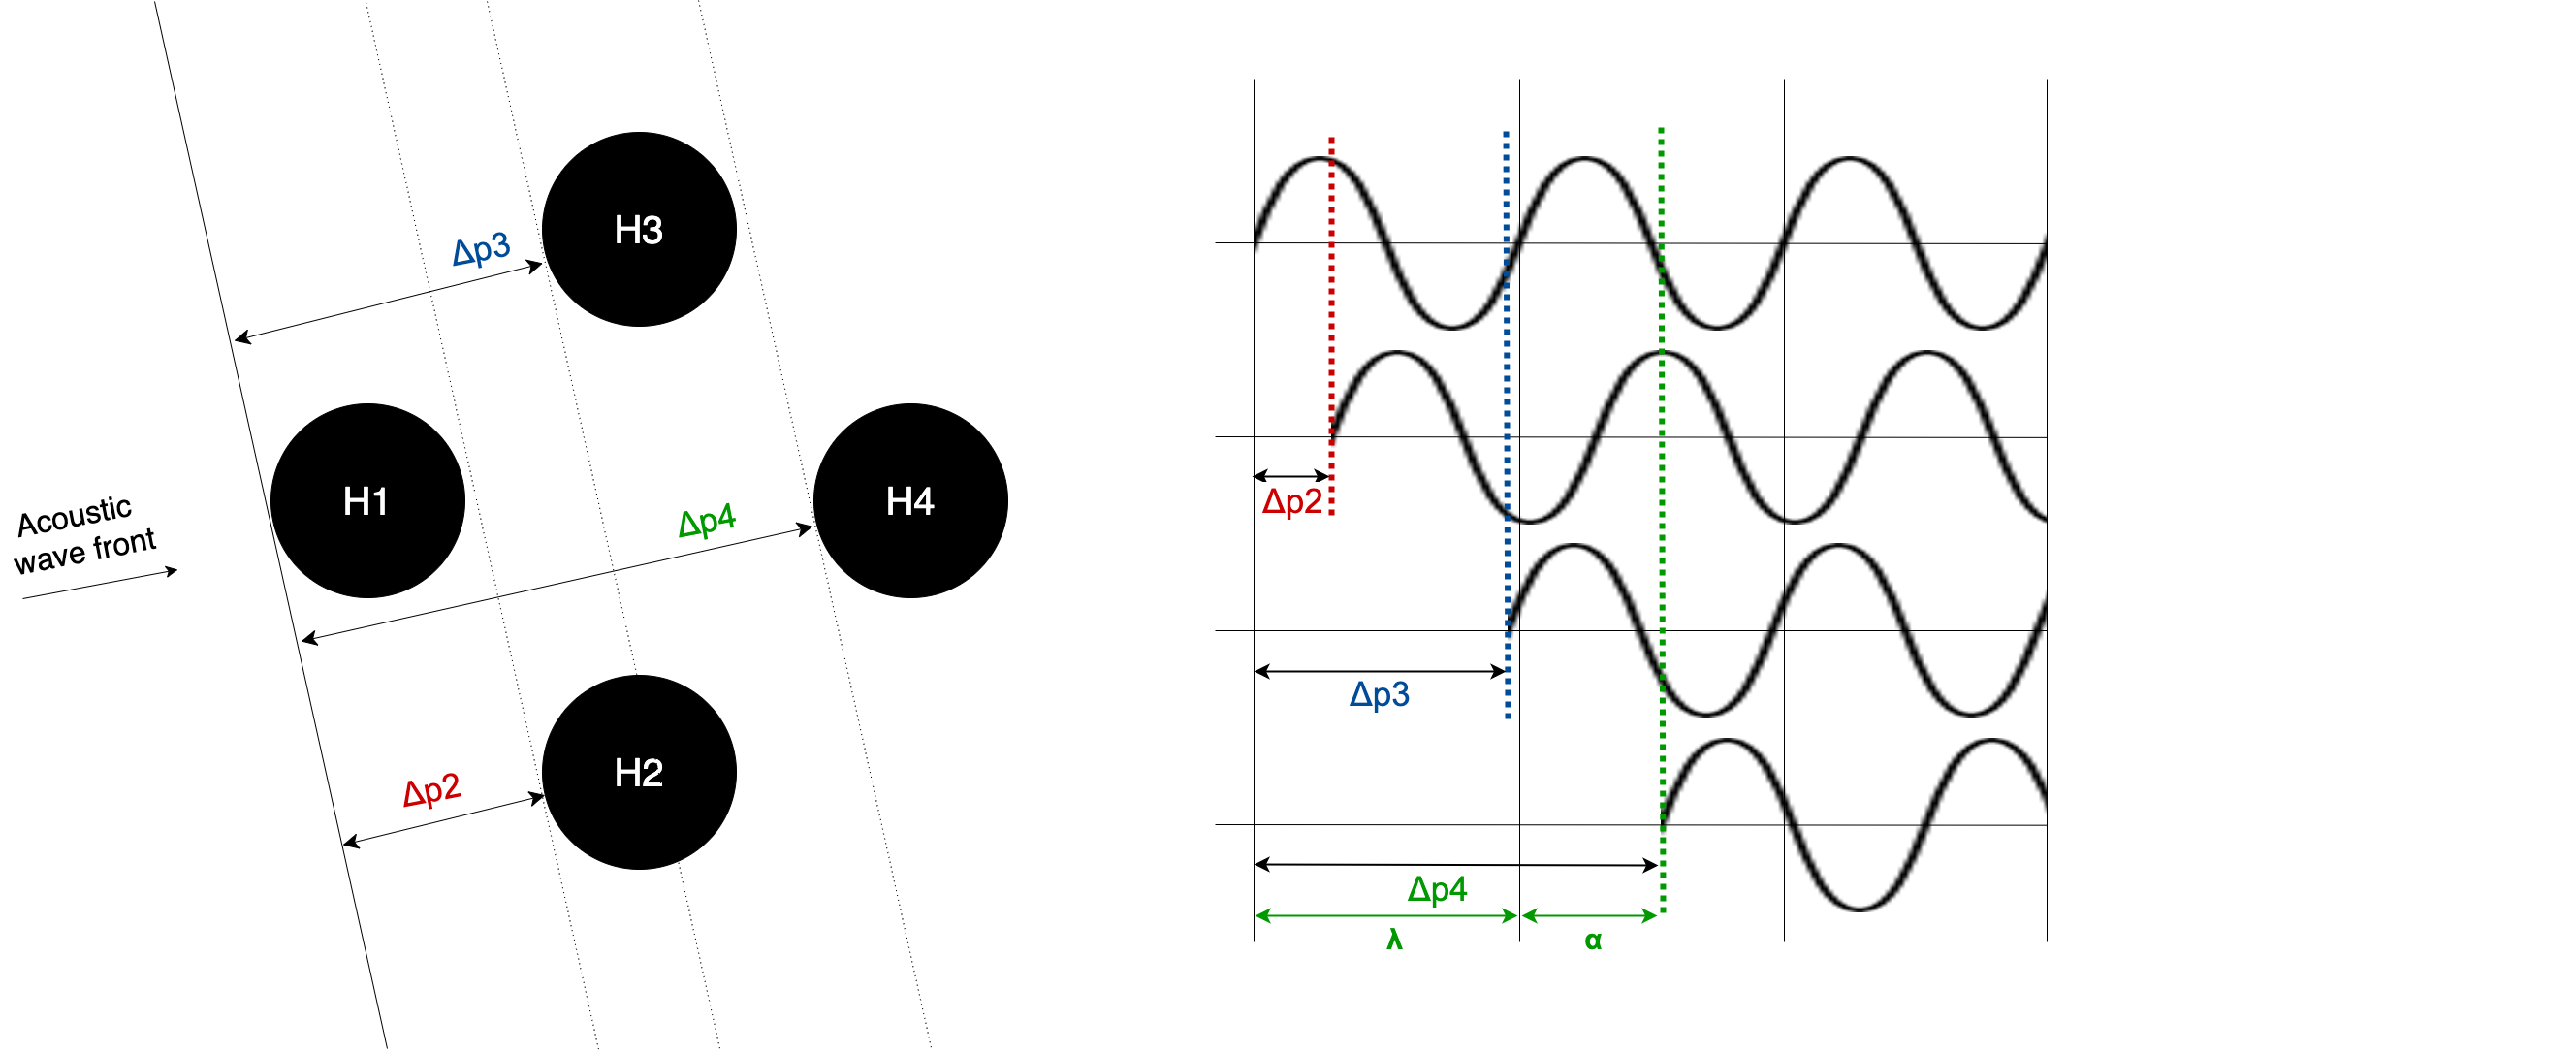
\includegraphics[width=1.2\textwidth]{figures/phase-diff}
	\caption{Phase difference to reference point and phase ambiguity}
	\label{fig:phasediff}
\end{figure}

For this reason, it is crucial to consider that the phase difference is given by the obtained phase value added by the number of periods ahead from the considered reference period.

In the system under study, the sent signals work with a operation frequency of 24.4 $kHz$. The corresponding signal period is $T = \frac{1}{24400} $ seconds which, considering the underwater acoustic speed \textit{c} equal to a standard 1500 $m/s$, the wavelength is approximately equal to $\lambda = \frac{T}{c} = 6.1 cm$. Having this into consideration, after obtaining the time of arrival to each hydrophone given by the cross correlation instances, besides the reference one, it is possible to conclude if the phase shift is superior to one period by analyzing if the time difference is greater than the duration of one period \textit{T}. In figure \ref{fig:phasediff}, each mentioned time difference between $H_1$ and $H_2$, $H_3$ and $H_4$ is converted to the corresponding phase differences $\Delta p_2$, $\Delta p_3$ and $\Delta p_4$.

One possibility to solve phase ambiguity in this system would be to place the four hydrophones with a baseline spacing inferior to $\frac{1}{2}$ of a wavelength, since the maximum reached by phase difference is 180 degrees. This way it would be possible to immediately deduce the phase difference since it would always be contained in one period. However, positioning the hydrophones closer together leads to smaller  values,causing a consequent increase on the estimation error due to varying environment conditions (briefly enumerated in \ref{subsec: acoustic-channel}). Additionally, since the hydrophones to be used in this system have a corresponding diameter of roughly half of a wavelength, they would not allow to execute the mentioned configuration and so this possibility will not be contemplated.

In order to compensate this phase ambiguity, a simple relation was developed which allows to calculate the absolute time difference between the moment a signal is received by hydrophone A, $T_A$, and when the same signal is received by a further hydrophone B, $T_B$. Figure \ref{fig:ambiguity} illustrates this association, where the represented sinusoidal waves correspond to the same signal arriving at hydrophones A and B. This correspondence uses the time stamps obtained by the correlation peaks combined with the calculated phase difference, that is determined in parallel, so that the measurement is more accurate. Equation \ref{eq:phase-amb} translates this relation, where $t_1$ and $t_2$ are the correlation peaks obtained from the signal arriving at hydrophone A and B, respectively, and so by rounding for the next integer number the difference between the correlation peaks, $t_2 - t_1$, we will obtain in which period, $T$, of signal in A will the signal in B arrive. Then the measurement is improved by subtracting a phase difference, $\theta_B - \theta_A$, so that the instant in which the signal is detected in hydrophone B can be defined. 

\begin{figure}[!htbp]
	\centering
	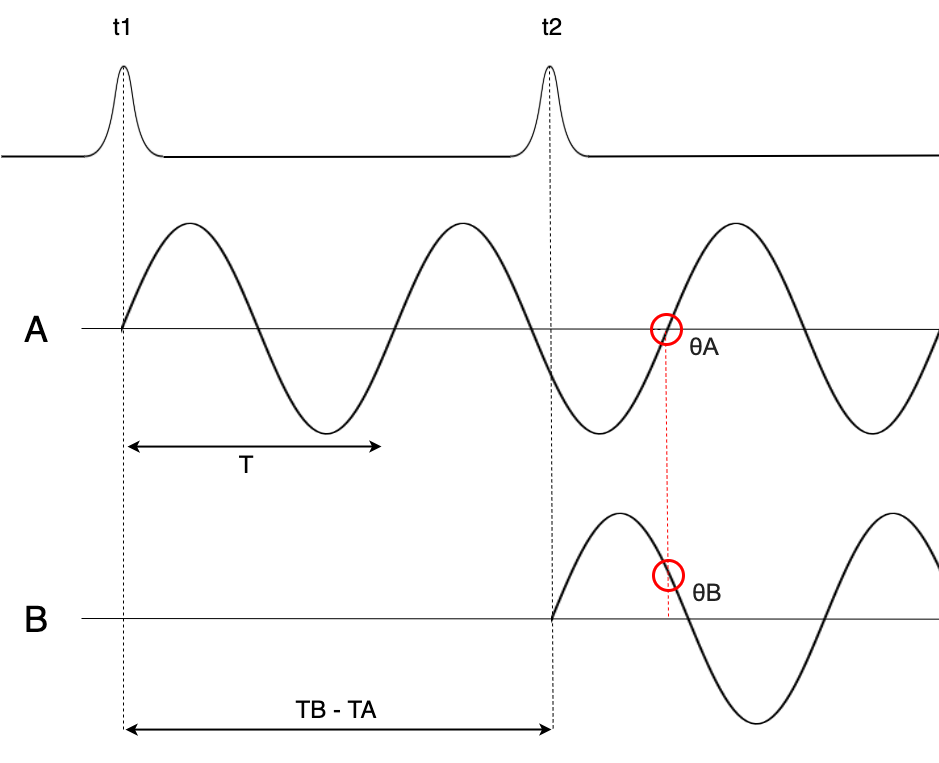
\includegraphics[width=0.6\textwidth]{figures/ambiguity}
	\captionsetup{justification=centering,margin=2cm}
	\caption{Ambiguity correction through correlation and phase difference}
	\label{fig:ambiguity}
\end{figure}

\begin{eqnarray}
& T_B - T_A = round(\frac{t_2-t_1}{T}) - (\theta_B - \theta_A)
\label{eq:phase-amb}
\end{eqnarray}

\subsubsection{Hydrophone position in relation to ToA}
To better understand the location estimation of an acoustic source in relation to the position of a pair of hydrophones, we can initially adopt the two dimensional scenario of figure \ref{fig:hyper}. 

Considering two hydrophones at known relative positions $(-f,0)$ and $(f,0)$, we can model all possible acoustic source locations for a specific ToA through hyperbolas. This is due to the fact that, by definition, the sum of the distances from the focus of each hyperbole, where each hydrophone is placed, to any point of the hyperbolic geometry corresponds to a constant value. 
This means that, in figure \ref{fig:hyper}, any point $(x,y)$ that is contained in the hyperbole corresponds to a constant $|d_2-d_1|$ value which, after some formulation, is in fact equal to $2*v$ or the distance between the vertexes of each hydrophone's hyperbola. Therefore, it is possible to trace a hyperbole that represents the positions of the target in space both based on their distance and the signal's ToA. In the exceptional case where $d_3=d_4$, we can observe that the possible positions are represented by an equidistant straight line to each hydrophone, such as the y axis.

\begin{figure}[!htbp]
	\centering
	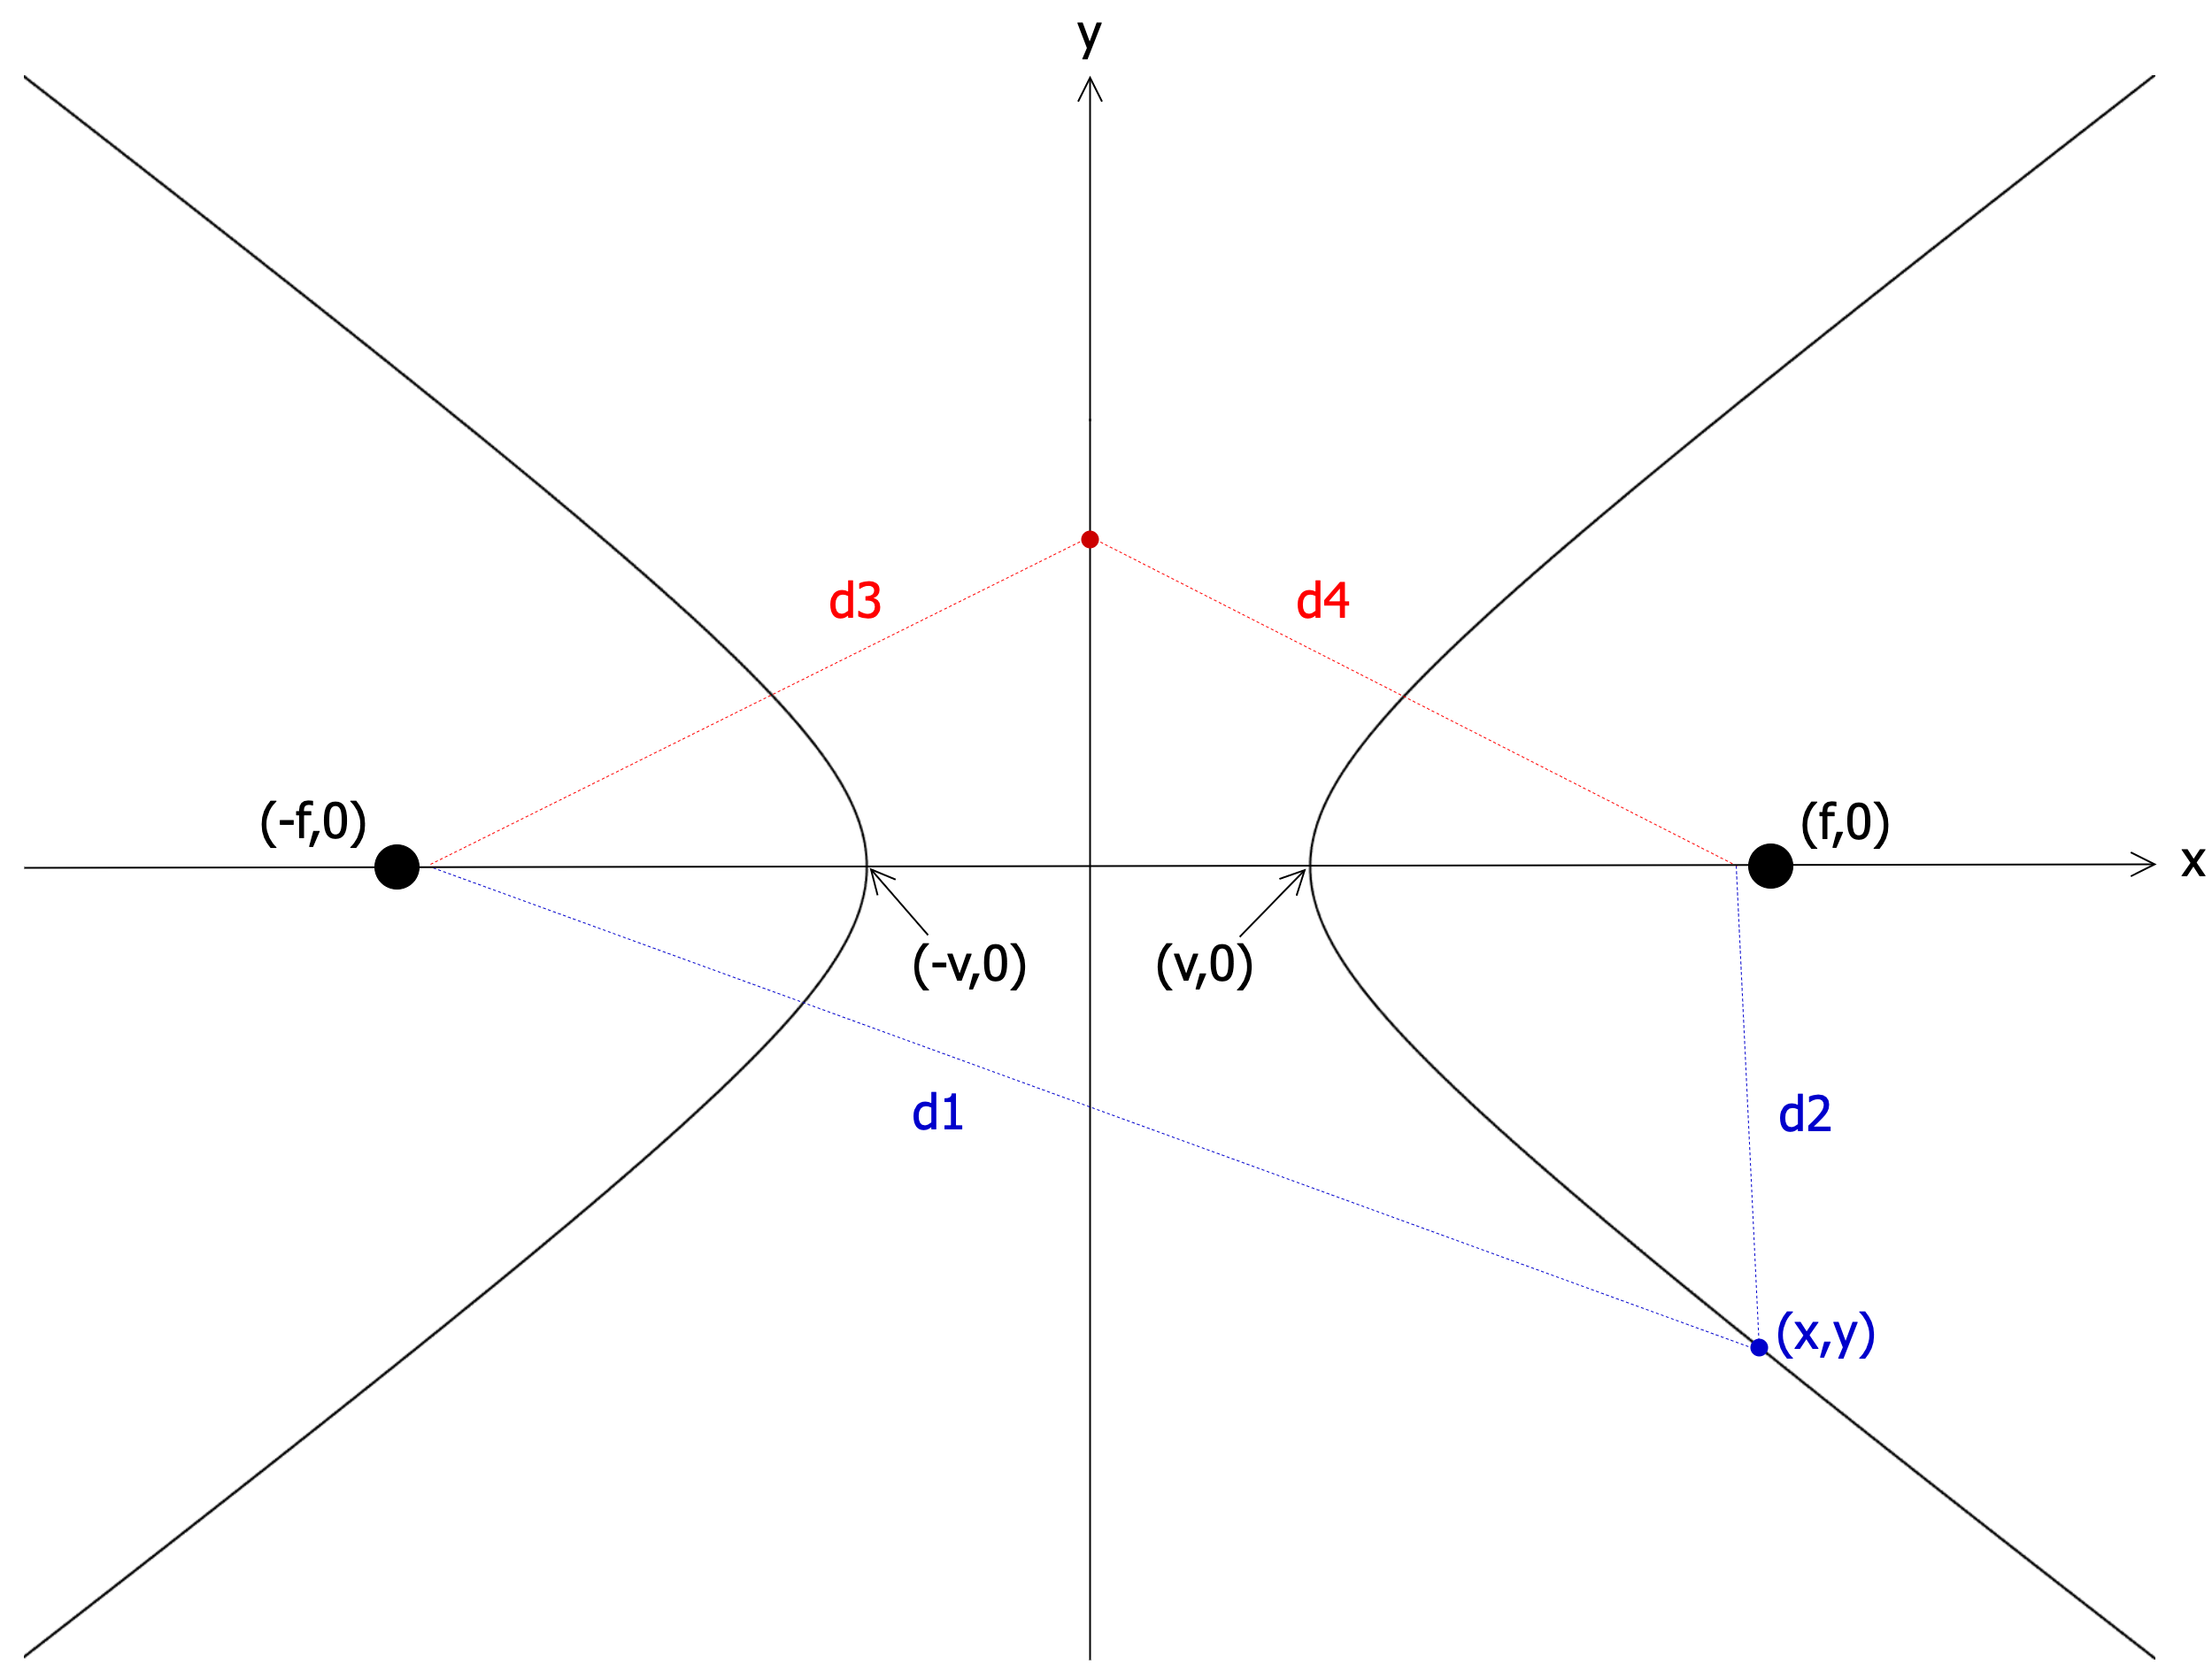
\includegraphics[width=0.8\textwidth]{figures/hyperbole-dist}
	\captionsetup{justification=centering,margin=2cm}
	\caption{Hyperbolic representation of acoustic source position possibilities in relation to ToA to two hydrophones}
	\label{fig:hyper}
\end{figure}

\subsubsection{ToA approximation} \label{subsubsec:toa-approx}

In order to estimate the location of an acoustic source we take into account the phase differences between each pair of hydrophones, carefully explained in section \ref{subchap:HDL module}. These phase differences can be translated into periods of the signal which combined with the ToA obtained from correlation of arriving acoustic signals are equivalent to relative distances.

Following the previous idea, it is possible to model the distance of one sensor to the target based on the known distance of a second sensor to the same target. 
This is to say that for two sensors with known relative positions where hydrophone 1 is the closer to the target, the distance from hydrophone i to the target, $D_i$, can be expressed as the distance of hydrophone j to the target, $D_j$, added by the time difference of arrival, $\Delta t_{ij}$, multiplied by the propagation velocity, $c_s$. Overall, this relationship is declared in equation \ref{eq:dist_to_target}.

\begin{eqnarray}
& D_i = D_j + \Delta t_{ij} * c_s
\label{eq:dist_to_target}
\end{eqnarray}

Therefore, the same logic can be applied for multiple hydrophones. In the present work, in which it is considered a system with four hydrophones, a synchronization mechanism allows to determine the signals' ToA between the transceiver and the hydrophones. However, in order to simplify the synchronicity and decrease errors that arise from it, the module that precisely computes the phase differences of the received signal in the hydrophones is used so that is possible to apply the relationship in \ref{eq:dist_to_target}. Consequently, a better angle of arrival estimation can be achieved when using this approximation than if all four times of arrival are used for the same purpose.

\subsubsection{Doppler Effect}

The implemented process uses the information of the transmitted signal's operating frequency in order to compute the phase differences and determine the overall times of arrival. However, in real scenarios the environmental conditions can distort this frequency between the source and the receiver. In the present study, since the vehicle is predominantly moving, then the Doppler effect could influence the signal's frequency, leading to erroneous calculations.

In order to evaluate if the Doppler effect influences the system, it is possible to calculate which is be the frequency deviation observed for a known relative speed between vehicles. Considering that the relative speed between the transmitter and the receiver is denoted as $relative\_speed$ and using a fixed sound speed, $c_s$, with a determined frequency of the transmitted signal, the relation \ref{eq:doppler} can be established. 

\begin{eqnarray}
&freq\_deviation = \frac{relative\_speed}{c_s} \times signal\_freq
\label{eq:doppler}
\end{eqnarray}

Therefore, considering the frequency of the signal equal to $24.4kHz$ and a $c_s$ of $1500 m/s$, it is observable that the frequency deviation will be dependent on the relative speed. Considering a transmitter that is static and a typical value for the navigation velocity of an AUV around $2 m/s$, which results in a frequency deviation of approximately $32.5Hz$. This allows to consider the Doppler effect negligible in this case.

A way to prevent this deviation is to integrate a frequency detector which senses the relative navigation speed in real time and adapts the used frequency. This mechanism is not integrated in the present research work.

%-------------------------------------------------------------------------------------
%-------------------------------------------------------------------------------------

\subsection{Monte Carlo estimator based on TDoA} \label{subsec:estimator}

The goal of the first proposed method is to estimate the position of an acoustic source in relation to known positions of a configuration of sensors, in a system of geometric axes with a defined origin. For this purpose, the logic employed is based on vector algebra with other physical considerations, detailed in the present subsection. 

Figure \ref{fig:AoA-init} represents the schematic of a considered scenario, where four hydrophones are placed in known relative positions in space and the origin of the axis is set on the body of the AUV or an alternative fixed structure. Then $r_i$ is defined as the vector that connects the origin of the axis to hydrophone $i$ and $rr_i$ defines the vector that connects hydrophone $i$ to the acoustic source. The black cross represents the acoustic source which is located somewhere in space. At last, the subtraction of the mentioned vectors is equal to $r$, according to \ref{eq:sum-vec}, which corresponds to the position of the acoustic source in relation to the origin of the axis and, overall, it is the variable that the method aims to determine.

\begin{eqnarray}
	& r_i = r + rr_i
	\label{eq:sum-vec}
\end{eqnarray}

\begin{figure}[!htbp]
	\centering
	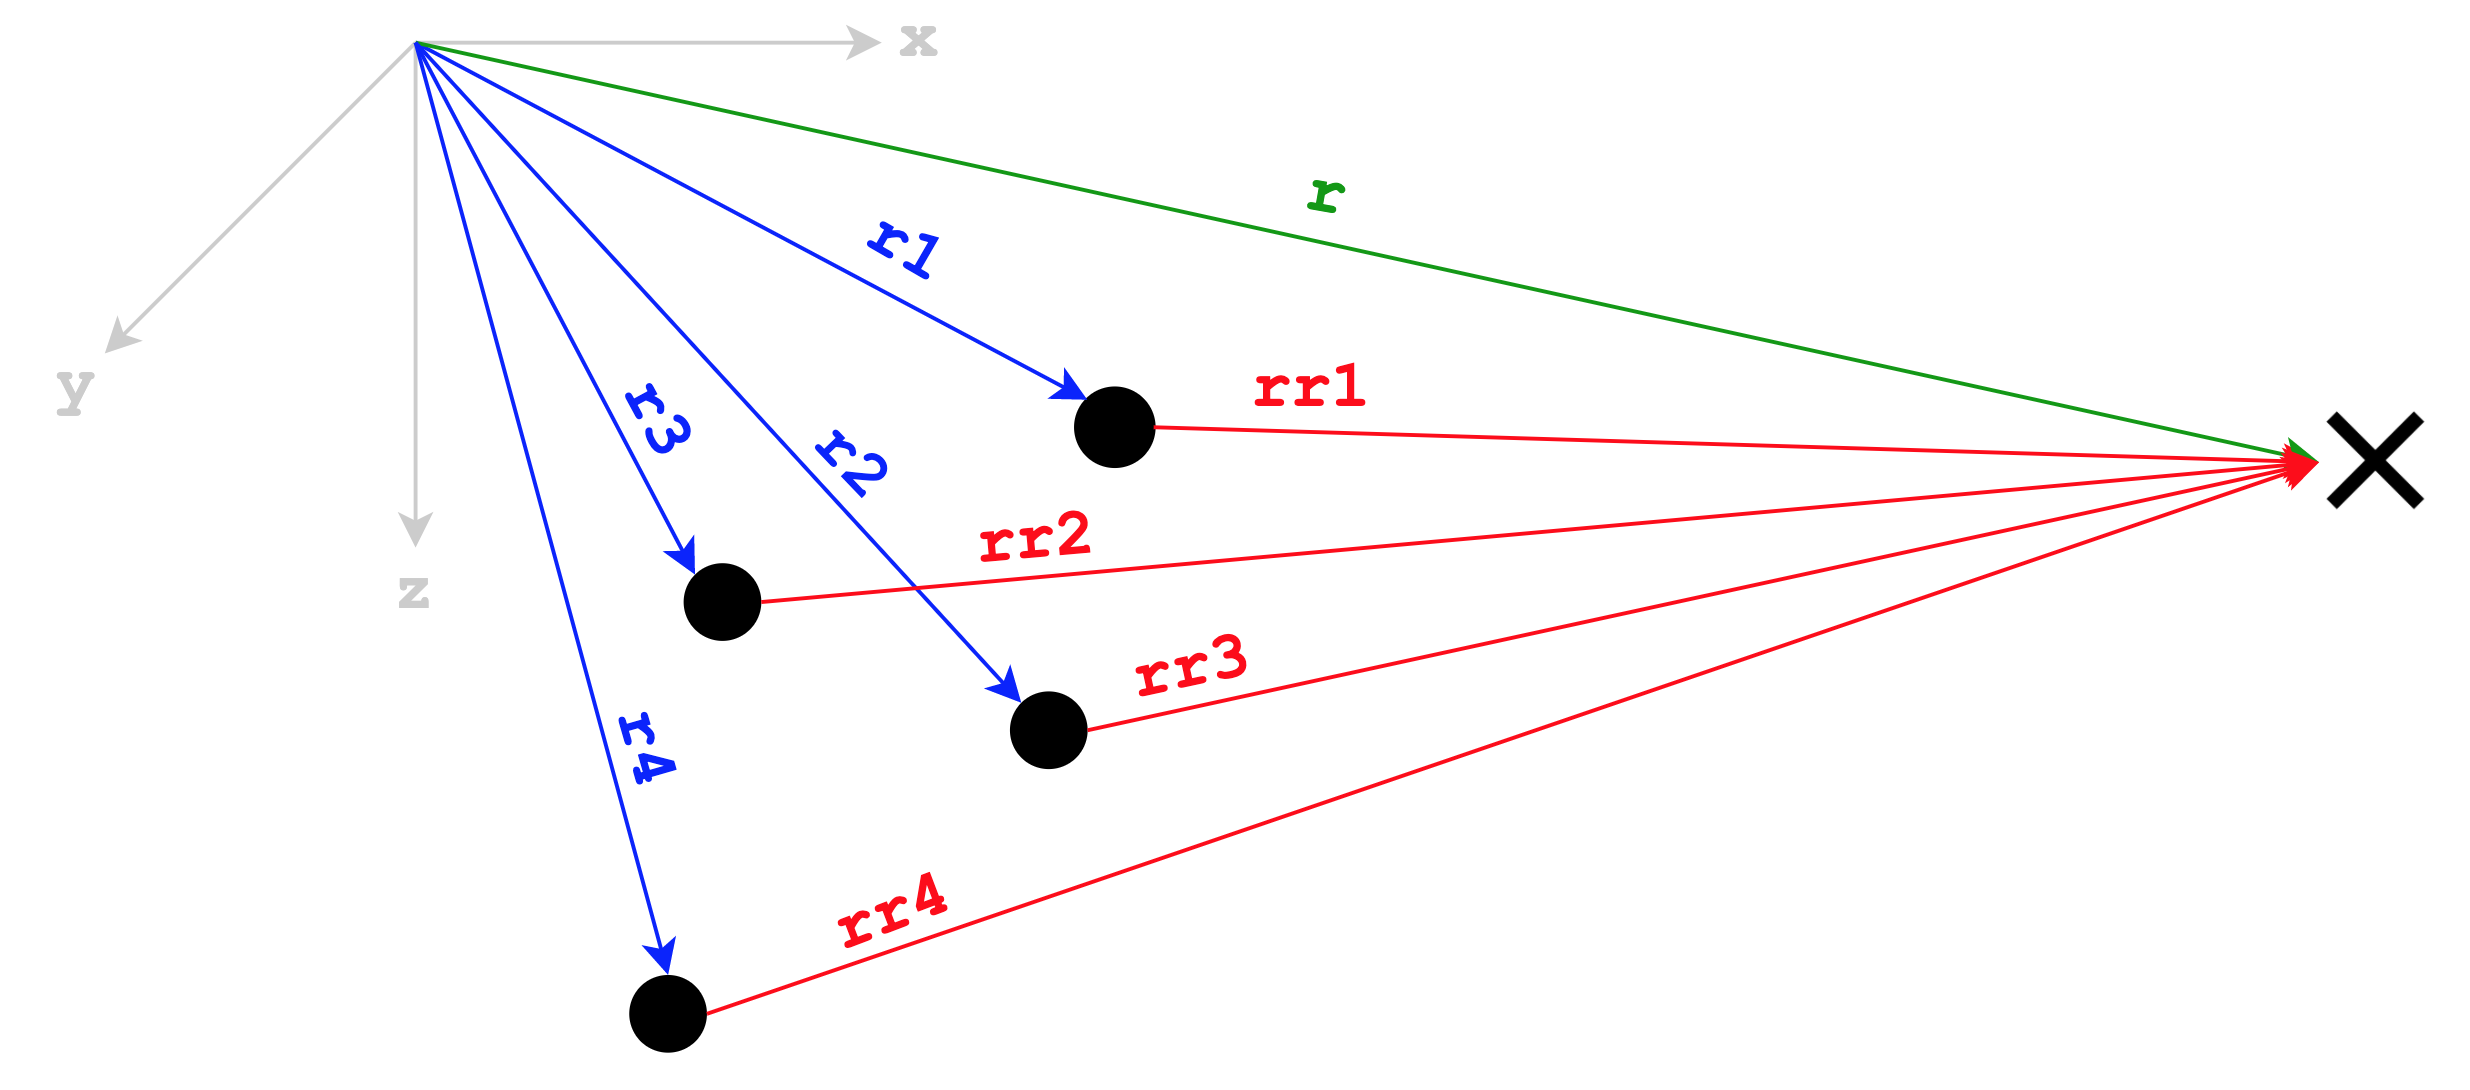
\includegraphics[width=0.8\textwidth]{figures/AoA-init}
	\captionsetup{justification=centering,margin=2cm}
	\caption{Considered scheme for angle of arrival estimation}
	\label{fig:AoA-init}
\end{figure}

Then we can define the times of arrival to each hydrophone as \ref{eq:toa-4h}, where $t_0$ is the absolute time of emission, $c_s$ is the underwater sound speed and $\rho_i$ is the norm of $rr_i$, \ref{eq:rho}, which translates to the distance from hydrophone $i$ to the acoustic source. 

\begin{eqnarray}
	& t_i = t_0 +  \frac{\rho_i}{c_s}
	\label{eq:toa-4h}
\end{eqnarray}

However, as explained previously, instead of using the absolute ToA in each hydrophone by computing the expression \ref{eq:toa-4h} for each of them, it can be expressed as a function of a single reference ToA. A simple logic was applied in order to determine this reference hydrophone, which starts by identifying the closest to the acoustic source. This allows to obtain all relative times of arrival by adding the defined reference time to each  between a hydrophone and the reference one. This is achieved by analyzing the  of each pair, $ \Delta t_{ij}$, for all possible combinations of two among four hydrophones, making up a total of six combinations. Considering each hydrophone pair $ij$ with $i, j= \{1,2,3,4\}$ :

\begin{itemize}
	\item if $ \Delta t_{ij}$ is positive, then hydrophone $i$ is closer to the acoustic source
	\item if $ \Delta t_{ij}$ is negative, then hydrophone $j$ is closer to the acoustic source
	\item if $ \Delta t_{ij}$ is zero, then $i$ and $j$ hydrophones are equidistant to the acoustic source
\end{itemize}

Considering these relations, it is possible to compose a vector that accumulates the closer hydrophone between each pair for a certain position of the acoustic source. Extracting the mode of this vector will then return the chosen hydrophone in most cases and therefore the overall closer to the acoustic source. If the closer hydrophones are the equidistant to the source, then it is indifferent which one is selected.  

Thereafter, recalling expression \ref{eq:dist_to_target}, it is possible to write \ref{eq:toa_relation2}, \ref{eq:toa_relation3} and \ref{eq:toa_relation4} which translate the used relations, where  the chose reference sensor is hydrophone 1, for the purpose of exemplification.

\begin{eqnarray}
	& T_2 = T_1 + \Delta t_{12} * c_s
	\label{eq:toa_relation2}\\
	& T_3 = T_1 + \Delta t_{13} * c_s
	\label{eq:toa_relation3}\\
	& T_4 = T_1 + \Delta t_{14} * c_s
	\label{eq:toa_relation4}
\end{eqnarray}

If then the distance $\rho_i$ is raised to the power of two, we know that $||rr_i||^2 = r_i^{T}r_i$, which allows to deduce equation \ref{eq:rho1} after some mathematical manipulation. Considering $\rho_i$ a physical distance, it is also possible to express it trough equation \ref{eq:rho2}, which uses the speed of propagation underwater multiplied by the ToA of the signal from the acoustic source to hydrophone $i$.

\begin{eqnarray}
	& \rho_i = ||rr_i|| 
	\label{eq:rho}\\
	&\rho_i^{2} =  r^{T}r + 2r^{T}r_i + r_i^{T}r_i
	\label{eq:rho1}\\
	&\rho_i^{2} = c_s^{2} (t_i-t_0)^{2}
	\label{eq:rho2}
\end{eqnarray}

Since two distinct relations are defined for $\rho_i^{2}$, then it is possible to consider the algebraic expressions as equivalent, thus forming a single equation to be resolved with only one unknown variable. After some mathematical manipulation, the matrix relation \ref{eq:AoA-matrix} is achieved, where $r$ is isolated and can be estimated.

\begin{eqnarray}
	\begin{bmatrix}
		1 & 2\: r_i^{T}
	\end{bmatrix}
	\begin{bmatrix}
		r^{T} r \\
		r
	\end{bmatrix}
	=  
	\begin{bmatrix}
		c_s^{2} (t_i-t_0) - r_i^{T} r_i
	\end{bmatrix}
	\label{eq:AoA-matrix}
\end{eqnarray}

In order to resolve this system of equations and isolate $r$, the least squares method is applied. If \ref{eq:AoA-matrix} is extended to the four considered hydrophones, we obtain matrix $A$ represented as \ref{eq:A} and $Y$ equivalent to \ref{eq:Y}. It is important to notice that the $A$ matrix has to be invertible, thus the rows which contain the chosen hydrophone configuration have to be linearly independent. The least squares method is then expressed as \ref{eq:least-square}, where $X \in \mathbb{R}^{4}$ holds the Cartesian result of $r$. As the method formulates four equations that are meant to calculate only three coordinates, $X$ will contain a fourth element that consists on a nonlinear component equivalent to $||r||^{2}$.

\begin{eqnarray}
	& A = 
	\begin{bmatrix}
		1 & 2\: r_1^{T}\\
		1 & 2\: r_2^{T}\\
		1 & 2\: r_3^{T}\\
		1 & 2\: r_4^{T}
	\end{bmatrix}
	\label{eq:A}
\end{eqnarray}

\begin{eqnarray}
	& Y = 
	\begin{bmatrix}
		c_s^{2}\: (t_1-t_0)^2 - r_1^{T} r_1\\
		c_s^{2}\: (t_2-t_0)^2 - r_2^{T} r_2\\
		c_s^{2}\: (t_3-t_0)^2 - r_3^{T} r_3\\
		c_s^{2}\: (t_4-t_0)^2 - r_4^{T} r_4\\
	\end{bmatrix}
	\label{eq:Y}
\end{eqnarray}

\begin{eqnarray}
	& X = (A^{T}*A)^{-1}*A^{T}*Y
	\label{eq:least-square}
\end{eqnarray}

After inferring the Euclidean vector $r$, it is possible to obtain both the bearing trough its direction, $\hat{\boldsymbol{r}}$, and the range through its magnitude, $||r||$.

%-------------------------------------------------------------------------------------
%-------------------------------------------------------------------------------------
\subsection{Monte Carlo estimator based on a plane wavefront}

The second explored method for evaluating sensor configurations' performance is a simpler approach than the previously proposed. It consists on an estimator which assumes that the signals' propagation can be approximated by a plane wavefront. When considering a planar wavefront approximation, it is assumed that the acoustic source is at a distance which is sufficiently larger than the relative distances between the hydrophones, for the signal to be considered to have a planar wavefront, thus the angle of arrival to each hydrophone being the same. This estimator is posteriorly integrated in a Monte Carlo approach to evaluate the configurations based on the obtained variance given different acoustic source positions.

Using a plane wavefront approximation means that, for signals arriving to the USBL system, it is assumed that the wavefront is coincident with a plane perpendicular to the direction of propagation, thus perpendicular to the angle of arrival as well. Figure \ref{fig:plane-wavefront} is illustrative of a plane wavefront arriving at two sensors. As represented, the angle or arrival is considered the same for every sensor, since the wavefront is the same as well, and it is possible to deduce the time of arrival to an hydrophone 1 by using the ToA to hydrophone 2 added by the time difference of arrival between 1 and 2. Therefore, it is also possible to obtain the estimation of the range, as it will be presented next.

\begin{figure}[!htbp]
	\makebox[\textwidth][c]{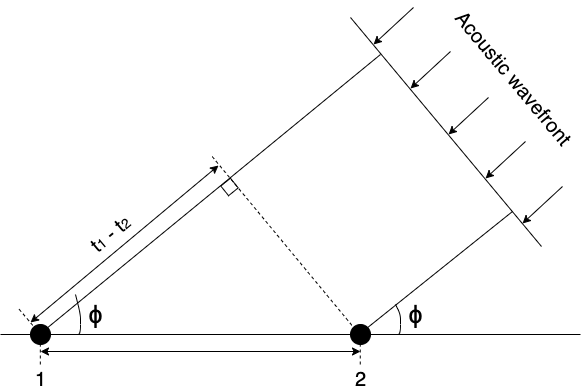
\includegraphics[width=0.7\textwidth]{figures/plane-wavefront}}
	\captionsetup{justification=centering,margin=2cm}
	\caption{Angle of arrival relation considering a plane wavefront}
	\label{fig:plane-wavefront}
\end{figure}

The estimator considers a USBL system composed by four sensors whose positions are previously defined. The time of arrival, $t_i$, to each hydrophone, $i$, is represented by expression \ref{eq:toa-planewave}. The considered $t_0$ is the absolute time of emission of the signal, which is acquired through a synchronization mechanism, the $s$ is the position of the transmitter, $a$ is referent to the mass center of the USBL's position, $r_i$ is the Cartesian coordinates of the hydrophone's position, $c_s$ is the sound speed and $e_i$ is an injected error that have the same characteristics expressed previously in \ref{subchap:acc-analy}.

\begin{eqnarray}
& t_i = t_0 + \frac{ ||s (a - r_i)|| }{c_s} + e_i
\label{eq:toa-planewave}
\end{eqnarray}

Due to the considered approximation to the plane wavefront, it is possible to calculate the range estimation, $\rho$, as a mean all propagation times multiplied by the sound speed,$c_s$, as in equation \ref{eq:range-planewave}. The $N$ represents the number of hydrophones.

\begin{eqnarray}
& \rho = c_s\ \frac{1}{N} \displaystyle\sum_{i=1}^{N} t_{i} - t_0
\label{eq:range-planewave}
\end{eqnarray}

Then a matrix $S$ is formulated as \ref{eq:S}, whose rows are the difference between the position of hydrophone 1 and the remaining three, and a $\Delta$ vector is expressed as \ref{eq:delta}, containing all combinations of TDOA between hydrophone 1 and the remaining.

\begin{eqnarray}
	& S = 
	\begin{bmatrix}
		r_1 - r_2\\
		r_1 - r_3\\
		r_1 - r_4
	\end{bmatrix}
	\label{eq:S}
\end{eqnarray}

\begin{eqnarray}
	& \Delta = 
	\begin{bmatrix}
		t_1 - t_2 \\
		t_1 - t_3 \\
		t_1 - t_4 
	\end{bmatrix}
	\label{eq:delta}
\end{eqnarray}

Taking into account the defined $S$ and $\Delta$, the signal's angle of arrival can be calculated from the direction of the signal, $d$, obtained from the least squares expression \ref{eq:direction-plane-wavefront} \cite{estim-plane-wavefront}. Since there are only three equations to estimate three coordinates, then the expression is linear. 

\begin{eqnarray}
& d = c_s \; (S^{T}S)^{-1} \; S^{T} \Delta
\label{eq:direction-plane-wavefront}
\end{eqnarray}

Having calculated the range $\rho$ and the direction $d$, the estimate of the transmitter position is given by the multiplication of these variables.

Finally, the plane wavefront estimator was integrated in a Monte Carlo method in order to execute multiple estimations of various transmitter positions, $s$, for a specific sensor configuration, so that it is possible to draw conclusions on its performance.

%------------------------------------------------------------------------------------
%-------------------------------------------------------------------------------------
\subsection{Fisher Information Matrix} \label{sucsec:FIM}

The Fisher Information Matrix (FIM) serves to quantify the information that an observable variable is capable of returning to an estimator. This concept is then integrated in the Crámer-Rao lower bound, which is a method that expresses the variance lower bound that a sensor configuration is capable of achieving. Unlike the two previously presented processes, the Crámer-Rao bound is independent from the used estimator, as it assumes a linear estimator that is efficient and unbiased.

The fundamental thought process and mathematical notation previously used in \ref{sec:cramer} are applied in the procedure that will be explained next.

The implementation of the Crámer-Rao bound method can be essentially partitioned in four steps:

\begin{enumerate}
	
	\item Formulate the observations vector
	\item Calculate the Fisher Information Matrix (FIM)
	\item Calculate the determinant of FIM 
	\item Apply optimality criteria to draw conclusions
	
\end{enumerate}

In this thesis, the number of used hydrophones per estimation is four, so all expressions will be presented for this case.

Firstly, the observation vectors are formulated based on an initial time of arrival $t_0$, which is given by a synchrony mechanism integrated in the global communication system, and the time of arrival based on the vectors that connect the hydrophone positions, $r_i$, to the transmitter, $s$. For a more realistic approach, it is also considered an added noise component that can be approximated to a Gaussian distribution $n_i \sim \mathcal{N}(\mu,\,\sigma^{2})$. 

The four observations vectors are then expressed as \ref{eq:obs-my1} to \ref{eq:obs-my4}.

\begin{eqnarray}
	t_1 = t_0 + \frac{s - r_1}{c} + n_1 \\
	\label{eq:obs-my1}
	t_2 = t_0 + \frac{s - r_2}{c} + n_2 \\
	\label{eq:obs-my2}
	t_3 = t_0 + \frac{s - r_3}{c} + n_3 \\
	\label{eq:obs-my3}
	t_4 = t_0 + \frac{s - r_4}{c} + n_4 
	\label{eq:obs-my4}
\end{eqnarray}

Then, addressing the second step, all conditions are set to calculate the FIM,  $I(d) \in \mathbb{R}^{3x3}$. In order to do so, if d$_{i}$ = $|| s - r_{i} ||$ is the distance between each sensor and the source, the gradient of the observations vector can be expressed as shown in \ref{eq:grad_fisher}.

\begin{eqnarray}
	\nabla_{d}t(d) = \frac{1}{c} 
	\begin{bmatrix}
		\frac{d_1^T}{||d_1||} \\ 
		\addlinespace
		\frac{d_2^T}{||d_2||} \\
		\vdots \\
		\addlinespace
		\frac{d_N^T}{||d_N||}
	\end{bmatrix}
	\label{eq:grad_fisher}
\end{eqnarray}

Additionally, the added noise component is present in the covariance matrix, represented as \ref{eq:covariance}, which integrates the FIM equation.

\begin{eqnarray}
	& \Sigma = 
	\begin{bmatrix}
		\sigma_1^2 & 0 & 0 & 0 \\
		0 & \sigma_2^2 & 0 & 0 \\
		0 & 0  & \sigma_3^2  & 0 \\
		0 & 0 & 0 & \sigma_4^2 
	\end{bmatrix}
	\label{eq:covariance}
\end{eqnarray}

Overall, the conditions to obtain the FIM matrix are established and, after some mathematical formulation, it can be expressed as \ref{eq:final-fisher}. This function can be validated by a similar study made on TOA based optimal positioning \cite{cramer-bruno}.

\begin{eqnarray}
	I(d) = \frac{1}{c^2} 
	\begin{bmatrix}
		\sum_{n=1}^{N} \frac{d_i d_i^T}{||d_i||^2} \frac{1}{\sigma_i^2}\\
	\end{bmatrix}
	\label{eq:final-fisher}
\end{eqnarray}

The final step is to calculate the determinant and find its relation to the volume of the \textit{uncertainty ellipsoid}. As mentioned before, in \ref{sec:cramer}, the Fisher Information Matrix determinant returns a deterministic value that represents the quantity of information which can be obtained and, therefore, the objective is to maximize it by respecting the condition $argmax \; det(I(d))$.

\subsubsection{Optimality criteria}

In order to evaluate the obtained values, several different optimality criteria can be applied. Considering similar applications in literature, the criterion that  the most relevant for the present case is the E-optimality, which minimizes the largest eigenvalue of the inverted FIM.

The FIM can be associated with a physical meaning, more specifically an uncertainty volume that characterizes the variance that a specific configuration can achieve for an estimate. In an initial approach the ellipsoid was not considered and instead an uncertainty sphere was analyzed. The radius of the uncertainty sphere, $u_{sphere}$, is expressed as \ref{eq:det-sphere}, which relates the three ellipsoid axis into a single mean radius that originates a figure of the same volume.

\begin{eqnarray}
	& u_{sphere}(d) = \sqrt[2]{\sqrt[3]{det(I(d)^{-1})}}
	\label{eq:det-sphere}
\end{eqnarray}

In this situation, the optimization objective is expressed as $argmin u_{sphere}(d)$, which indicates that the error that originates a certain uncertainty radius is minimal.

In a further analysis, the uncertainty ellipsoid is calculated using \ref{eq:det-ellip}. The squared eigenvalues of the inverse of the FIM indicate the length of each of the three ellipsoid axis and the eigenvectors specify the direction of each axis. An eigenvector that is associated with the smaller eigenvalue indicates the direction in which there is less uncertainty and, equivalently, an eigenvector whose eigenvalue is the larger represents the direction in which there is the biggest uncertainty. Consequently, the goal in this case is to minimize the maximum squared eigenvalue of the FIM inverse, $argmin \; max(\sqrt{eigenvalue})$.

\begin{eqnarray}
	& u_{ellipsoid}(d) = \sqrt[2]{eig(I(d)^{-1})}
	\label{eq:det-ellip}
\end{eqnarray}

Besides the E-optimality, several more criteria can be used in order to evaluate the performance of a specific hydrophone configuration, using the Fisher Information Matrix. The most common alternatives would be:
\begin{itemize}
	\item A-optimality: minimizes the trace of the inverse of the FIM, therefore seeks the minimum average variance of the estimates.
	\item D-optimality: minimizes the determinant of the inverse of the FIM, therefore the volume of the uncertainty sphere. However, this can be misleading since the information obtained for one direction can be much larger than the other directions, constituting a large FIM determinant which is not representative of the full estimation.
\end{itemize}

%-------------------------------------------------------------------------------------
%-------------------------------------------------------------------------------------

\subsection{Performance comparison between methods} \label{subsec:perform-compar-meth}

Upon presenting the theoretical details behind the three considered methods for evaluating configurations' performance, a further functional study will be presented through simulation results. 

Throughout the functional demonstrations, three different hydrophone configurations are considered, A, B and C defined in \ref{tab:configs_test1}, where the columns $r_{Ai}$, $r_{Bi}$ and $r_{Ci}$ contain the position's coordinates of each hydrophone $i$.

\begin{table}[!htbp] %use H to adjust
	\begin{center}
		\begin{tabular}{ l | c c c c | c c c c | c c c c}
			%\hline
			%\multicolumn{1}{c|}{} & \multicolumn{4}{c|}{A} & \multicolumn{4}{c|}{B} \\
			\toprule
			% \cline{2-9}
			\multicolumn{1}{c|}{} & $r_{A1}$ & $r_{A2}$ & $r_{A3}$ & $r_{A4}$ & $r_{B1}$ & $r_{B2}$ & $r_{B3}$ & $r_{B4}$ & $r_{C1}$ & $r_{C2}$ & $r_{C3}$ & $r_{C4}$ \\
			\midrule
			\multirow{1}{0.5em}{x} 
			& 0.02 & 0.02 & 0 & 0 & 0.1 & 0.1 & 0 & 0 & 0.1 & 0 & 0 & 0  \\
			%\hline 
			\multirow{1}{0.5em}{y} 
			& 0 & 0 & 0.1 & -0.1 & 0 & 0 & 0.1 & -0.1 & 0 & 0 & -0.0707 & 0.0707 \\
			%\hline 
			\multirow{1}{0.5em}{z} 
			& 0.1 & -0.1  & 0 & 0 & 0.1 & -0.1  & 0 & 0 & 0 & 0.1 & -0.0707  & -0.0707\\
			\bottomrule 
		\end{tabular}
		\caption{Hydrophone configurations used for accuracy tests}
		\label{tab:configs_test1}
	\end{center}
\end{table}


For testing both estimators, a methodology was formulated in order to evaluate the accuracy that they can achieve in defined circumstances. This approach is a Monte Carlo algorithm which allows to reiterate the estimation process according to the number of positions that are intended to be tested for a specific configuration, as well as create a series of repetitive calculations that allow to deduce the estimation error and turn the overall process more robust. For this initial study, the following conditions are considered: 

\begin{enumerate}[label=\alph*)]
	%--------------------
	\item \textbf{Sensor Configuration}  
	
	Each hydrophone configuration is analyzed individually. It is a parameter to be always defined and known from the begging of each simulation.
	
	%--------------------
	\item \textbf{Reference axis}
	
	The origin of the reference axis is defined at the center of mass of the structure where the hydrophones are fixed, which in this case is the AUV.
	
	%--------------------
	\item \textbf{Injected error} 
	
	In order to make the study more realistic, an $e_i$ error is added to the time differences of arrival, $ \Delta t_{ij}$. These errors are mutually independent and follow a Gaussian distribution with zero mean and a configurable variance of $\sigma^{2}$, i.e., $e_i \sim \mathcal{N}(0,\,\sigma^{2})$. 
	
	For the simulations performed in this project, a deviation of 5$^{\circ}$, or a window of $[-2.5^{\circ},2.5^{\circ}]$, in phase difference estimation of incoming singals was considered to be reasonable for an underwater navigation scenario. Therefore, since the specified period of the signal is $T = \frac{1}{24400}$ and one period corresponds to a 360$^{\circ}$ phase shift, then the 5$^{\circ}$ will be equivalent to $\frac{5^{\circ}}{360^{\circ}}*T$ which is approximately a deviation of $0.5\mu s$. Hence the considered standard deviation $\sigma$ of the error $e_i$ in the computed time differences of arrival is equal to $0.5\mu s$.
	
	Overall, the considered total time of arrival is equal to the measured time between the transmitter and the receiver through correlation, added by the computed time difference of arrival for a specific pair of hydrophones and the injected error $e_i$ in seconds.
	
	%--------------------
	\item \textbf{Acoustic source position} 
	
	The considered positions for the acoustic source, $s$, are originally defined in spherical coordinates, $s_{sph}$. Thus the norm, $n$, corresponds to the source's range in meters, whereas the azimuth, $\phi$, and elevation, $\theta$, define the angle of arrival of the received signal in degrees. Additionally, when these positions are mentioned in Cartesian coordinates throughout the document, they will be referenced as $s_{cart}$.
	
	Recalling the definition of spherical coordinates, it is known that for elevations of -90$^{\circ}$ or 90$^{\circ}$, the azimuth angle is meaningless and should not be considered. Since this system is affected by a Gaussian error, then the estimated azimuth angle is expected to return large errors not only for the absolute mentioned elevation values but for a considerable interval around it, dependent on the injected deviation. For that reason, the elevation values are limited to an interval between -80$^{\circ}$ and 80$^{\circ}$ so that the evaluated metrics present a result that is not so reflective of the errors originated from this phenomenon.
	
	The positions to be estimated are contained in a matrix with a number of columns equal to the number of positions and three rows consisting of its spherical coordinates. The matrix is arranged so that for each defined norm, the elevation component covers the interval [-80$^{\circ}$ to 80$^{\circ}$] in steps of one and, for each elevation value, the azimuth component covers the interval [-180$^{\circ}$, 180$^{\circ}$] in steps of one, forming partial spheres around the reference axis' origin.
	
	%--------------------
	\item \textbf{Propagation speed}
	
	In all performed simulations, the considered speed of sound is $1500 \; m/s$, which corresponds to the underwater propagation velocity of waves in typical conditions.
	
\end{enumerate}

Having the conditions enumerated, the logic of the algorithm occurs as follows. For every defined position of the acoustic source, $s$, a function that consists on the estimator is called, receiving as input the $s$, the positions of the hydrophone configuration, $r_i$, and an injected error in the . It then returns the estimated position of the source in Cartesian coordinates, $[x,y,z]$, and in spherical coordinates, $[n, \phi, \theta]$. As the position $s$ in Cartesian corresponds to the real value that is intended to be estimated, we can also obtain the real spherical coordinates by directly converting $s$ using the Cartesian to spherical relations in \ref{eq:cart2sph}.

\begin{eqnarray}
	\begin{cases} 
		n =  \sqrt{x^2 + y^2 + z^2}\\ 
		\phi  = arctan \frac{y}{x}\\ 
		\theta =  arctan \frac{\sqrt{x^2+y^2}}{z}
	\end{cases}
	\label{eq:cart2sph}
\end{eqnarray}

Consequently all conditions are met to analyze the achieved error in each coordinate by comparing the real position to the estimated values as \ref{eq:error1}, where the tested coordinates are $x, y, z, n, \phi$ and $\theta$.

\begin{eqnarray}
	&error_{coordinate} = |estimated_{coordinate} - real_{coordinate}|
	\label{eq:error1}
\end{eqnarray}

The metrics used to evaluate the quality of the estimator were :

\begin{itemize}
	\item \textbf{Mean squared error} (MSE): Incorporates both the variance and the bias of the estimator, indicating its overall quality
	
	\item \textbf{Standard deviation of the error} ($\sigma$) : Indicates how disperse are the estimates from the expected value
	
	\item \textbf{Minimum error ($min(e_i)$)} : Indicates the minimum error that is obtained by the estimator, thus the best absolute precision achieved
\end{itemize} 

\subsubsection{Functional analyzes of Monte Carlo TDoA estimator}

Since this Monte Carlo algorithm was developed for this specific application, then it is possible to test diverse parameters of the system in order to characterize it. Therefore, a series of detailed simulations were performed using the TDoA estimator to understand the behavior, capabilities and the impact of some design decisions on the overall accuracy.

To illustrate a scenario where this estimator is applicable, we can consider that a vehicle is moving towards an acoustic signal transmitter whose position is unknown. Imagining that the target is at a considerable distance, then the main focus is to achieve an optimal bearing estimation which provides a more direct path and saves resources. The range estimation serves as secondary measurement that indicates how near the vehicle is from the destination, so that it is possible to make control decisions such as moderate the navigation speed in the proximity of the target. For the reasons outlined, the study that follows presents a more thorough analysis of the azimuth and elevation errors. 

For the data visualization, two essential types of representation were developed :

\begin{itemize}
	\item A 2D static representation of the error per position $s$. The errors to be tested are coordinates $x, y, z$, norm, azimuth angle or elevation angle.
	
	\item A 3D map of the obtained error. The x-axis holds the azimuth angle in degrees, the y-axis holds the elevation angle in degrees and the z-axis represents the measurement of a chosen parametric error. This allows to visualize, for a chosen configuration, how the estimation quality evolves in space.
	
\end{itemize}

For the first simulation, configuration A is tested for the acoustic source positions $s$  previously described, in a total of 58121, with a norm equal to 10 meters. Upon simulation, it is possible to observe that the geometric symmetrical nature of the configuration leads to estimation error patterns. Accordingly, it is possible to characterize the tendency of the azimuth and elevation errors according to the range of spherical coordinates angles. Table \ref{tab:configA-tendency} summarizes these relations, where the arrows indicates if the error tendency is ascendant $\nearrow$ or descendant $\searrow$.

\begin{table}[!htbp] %use H to adjust
	\begin{center}
		\makebox[\textwidth]{
			\begin{tabular}{ c | c c c}
				%\hline
				\toprule
				\multicolumn{1}{c|}{} & Range & Azimuth error & Elevation error\\
				\midrule
				\multirow{4}{*}{Azimuth angle} 
				& $-180^{\circ}$ to $-90^{\circ}$ & $\nearrow$  & $\searrow$   \\  
				\cmidrule{2-4}
				&$-90^{\circ}$ to $0^{\circ}$ & $\searrow$  & $\nearrow$ \\ 
				\cmidrule{2-4}
				& $0^{\circ}$ to $90^{\circ}$ & $\nearrow$  &  $\searrow$  \\
				\cmidrule{2-4}
				& $90^{\circ}$ to $180^{\circ}$ & $\searrow$  & $\nearrow$ \\
				\midrule
				\multirow{2}{*}{Elevation angle} 
				&$-90^{\circ}$ to $0^{\circ}$ & exponential $\searrow$ & $\searrow$   \\ 
				\cmidrule{2-4}
				& $0^{\circ}$ to $90^{\circ}$ & exponential $\nearrow$  & $\nearrow$ \\
				\bottomrule 
		\end{tabular}}
		\caption{Azimuth and elevation errors slope tendency for configuration A}
		\label{tab:configA-tendency}
	\end{center}
\end{table}

By analyzing the collected information, it is possible to deduce that since the configuration's geometric center is located along the x-axis, then for elevation angles increasingly closer to $0^{\circ}$ the errors have a tendency to decrease. Moreover, adding the fact that the depth of the baseline along the x-axis is shorter then the remaining, it results in a better azimuth estimation and a worst elevation estimation near an azimuth angle of $180^{\circ}$ or $0^{\circ}$. Overall, the maximum achieved errors are: for azimuth error $\approx$ $7.55^{\circ}$, for elevation error $\approx$ $1.41^{\circ}$ and for norm error $\approx$ 0.25m, which corresponds to 2.5\% of error in norm estimation.

For the same conditions, the maximum resulting $x, y$ and $z$ errors are: for $x$ $\approx$ $0.28m$, for $y$ $\approx$ $0.037m$ and for $z$ $\approx$ $0.038m$. It should be pointed out that there is a higher error in the $x$ coordinate, which corresponds to the direction of the shorter baseline that consequently originates a greater uncertainty.

From this experiment, it was possible to collect the standard deviation and the minimum estimation error achieved for the azimuth and elevation angles, which are present further ahead in \ref{tab:azimuth-test1}. It should be noted that the chosen configuration A for the former analysis is by no means an optimal solution for the estimation. This particular layout was selected because it emphasizes several system responses to distinct configuration characteristics, allowing to understand how should them be adapt to achieve better results.

In order to further analyze the influence of the hydrophones placement in the estimation and which design choices lead to better estimations, two more scenarios are considered to test different aspects:

\begin{itemize}
	\item \textbf{Influence of range in estimation}: In order to compare the range influence on the estimation, a second simulation intends to test the same configuration for a norm of 100 meters. The azimuth and elevation estimations do not demonstrate any visible changes in terms of range and the norm error increases for a maximum of $2.65m$, which still corresponds to approximately 2.6\% error from the original norm. However, the $x, y$ and $z$ estimation demonstrate an error increase of about 10 times, since a small deviation in angle can correspond to a large difference in Cartesian coordinates. Nonetheless, for increasing ranges these errors stay proportional, so the error percentage is similar in any range. This phenomenon is illustrated in \ref{fig:cart-range}, where the error in $x$ is represented for all the tested positions that form spheres with norms equal to $10 m$, $100 m$ and $1000 m$. As it is observed, the errors increase proportionally with the norm.
	
	\begin{figure}[!htbp]
		\makebox[\textwidth][c]{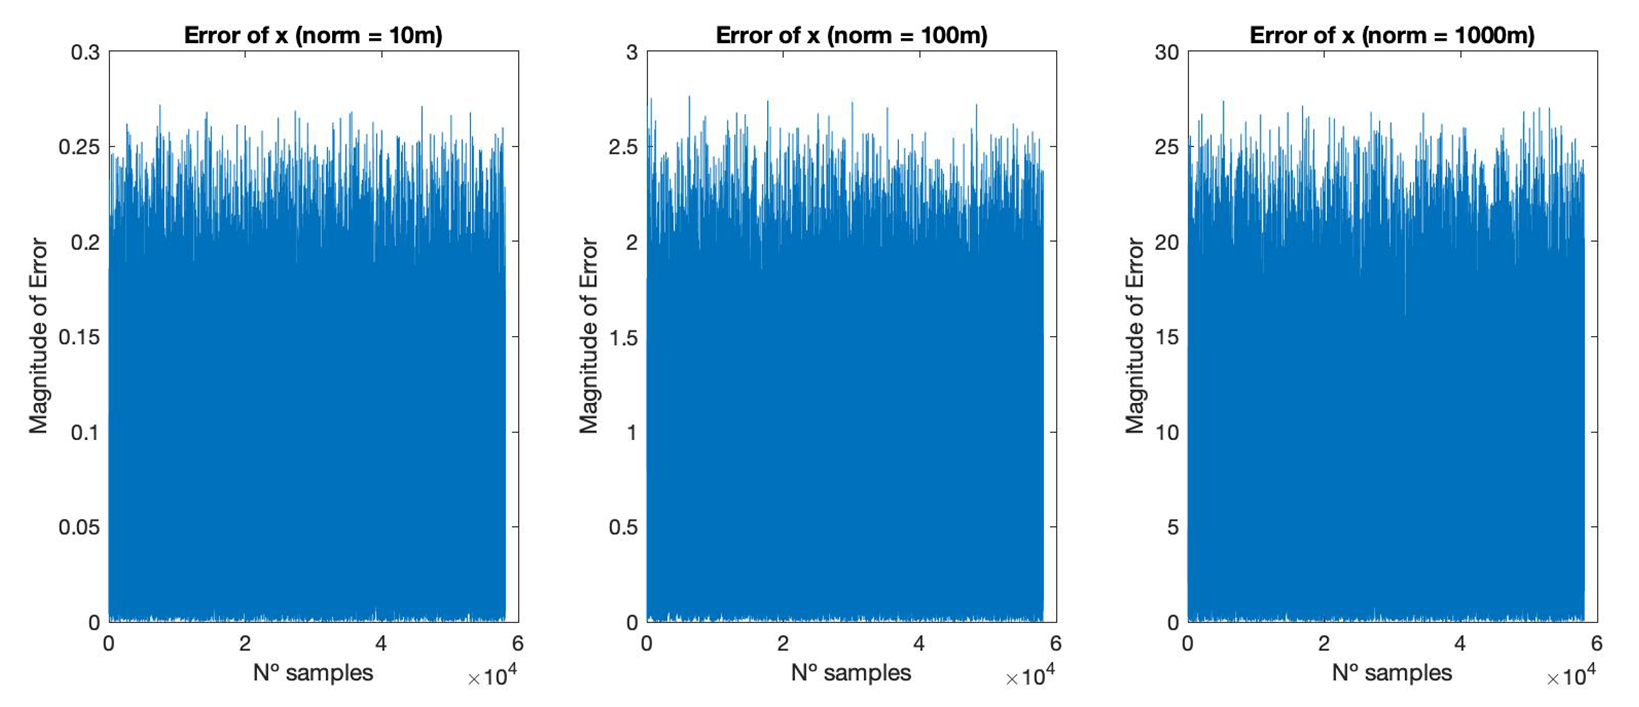
\includegraphics[width=1\textwidth]{figures/plot-cartesian-range}}
		\captionsetup{justification=centering,margin=2cm}
		\caption{Evolution of error in Cartesian coordinates for increasing norm}
		\label{fig:cart-range}
	\end{figure}
	
	\item \textbf{Increasing the shorter baseline}: Since there are some issues that can be observed due to the short baseline along the x-axis, a third simulation serves to understand the influence of increasing this baseline in the estimation. Therefore, the baseline is increased by employing configuration B. After the simulation, the errors decreased visibly, which are indicated in \ref{tab:tdoa-estimator-abc}.
\end{itemize}

After analyzing a specific configuration which demonstrate various limitation due to its arrangement design, it is desirable to compare it with different hydrophone placements. Therefore, table \ref{tab:tdoa-estimator-abc} contain the achieved results of MSE, standard deviation and minimum error for azimuth and elevation estimation in degrees, using norms equal to 10 and 1000 $m$ for configurations A, B and C. Configuration A represents an almost flat structure, configuration B is a variation of A with an increased depth and configuration C resembles an AUV shape. By inspection it is possible to conclude that configuration B returns the lowest standard deviation and MSE, as it is also the one with the larger baselines between sensors.

\begin{table}[!htbp] %use H to adjust
	\begin{center}
		\makebox[\textwidth]{
			\begin{tabular}{ c | c c | c c | c c}
				%\hline
				\toprule
				\multicolumn{3}{c|}{} & \multicolumn{2}{c|}{Azimuth} & \multicolumn{2}{c}{Elevation}  \\
				\midrule
				% \cline{2-9}
				\multicolumn{1}{c|}{Configuration} & Norm & MSE & Standard Dev & Minimum & Standard Dev & Minimum \\
				\midrule
				\multirow{2}{*}{A} &10 & 0.544 & 0.605 & 8.743$\times10^{-7}$ & 0.186 & 3.103$\times10^{-6}$\\
				%	&100 & 0.5465 & 0.6090 & 6.0529$\times10^{-6}$\\
				&1000 & 0.542 & 0.599 &  8.378$\times10^{-6}$ & 0.185 & 5.059$\times10^{-6}$\\
				\midrule	
				\multirow{2}{*}{B} &10 & 0.161 & 0.143 & 1.21$\times10^{-6}$ & 0.050 & 3.456$\times10^{-6}$\\
				&1000 & 0.161 & 0.144 & 1.494$\times10^{-6}$  & 0.050 & 4.910$\times10^{-7}$\\
				\midrule			
				\multirow{2}{*}{C} &10 & 0.230 & 0.213 & 1.305$\times10^{-5}$  & 0.067 & 2.790$\times10^{-5}$\\
				%	&100 & 0.2304 & 0.2119  & 4.3874$\times10^{-6}$\\
				&1000 & 0.223 & 0.212 & 4.096$\times10^{-6}$  & 0.066 & 4.394$\times10^{-6}$\\
				\bottomrule 
		\end{tabular}}
		\caption{Obtained errors for configurations A,B and C by TDoA estimator}
		\label{tab:tdoa-estimator-abc}
	\end{center}
\end{table}

Having explored the behavior of the estimator in specific conditions, there are still factors which were not discussed that may influence the system's performance or lead to an improvement. Therefore, four main ideas will be explored regarding the influence of the numeric quantization on the estimation accuracy, weather the absolute ToA is absolutely necessary for the position estimation, how is the estimates' dispersion for a specific position due to the injected error and the influence of increasing the baseline to the estimation accuracy.

\paragraph{a) Influence of numeric quantization on accuracy}

The first term to be analyzed is how much does the quantization of the calculations influence the obtained accuracy of the estimator. In order to analyze this, a simple adaptation was made to the numeric precision of the TDoA values that are input of the system. Instead of using the MATLAB precision of fifteen decimal places, the value was truncated to a specified number of decimal places, $\kappa$.
Since the time differences of arrival have magnitudes around microseconds, then initially they are multiplied by $10^6$ to avoid missing information. Then the relation \ref{eq:trucate} is applied resulting in a truncated value with $\kappa$ decimal places. Finally after the truncation, the value is converted again to seconds to be used in the algorithm.

\begin{eqnarray}
	&_{truncated} = \frac{round(*2^{\kappa})}{2^{\kappa}};
	\label{eq:trucate}
\end{eqnarray}

To evaluate the influence of the truncation in the estimation, configuration C is used to test a norm equal to 10. The original measurements are already represented previously. For a $\kappa$ of one decimal place, the azimuth standard deviation is 0.261 degrees, the elevation standard deviation is 0.087 degrees, the norm standard deviation is $0.014m$ and the MSE is 0.272. Overall, the estimation errors increase but, in practical terms, the truncation causes near to any difference in the estimation. 

Since one decimal place does not bring too much discrepancy, the limit case is tested where zero decimal places are considered. In this case, the azimuth standard deviation is $0.416^{\circ}$, the elevation standard deviation is $0.136^{\circ}$, the norm standard deviation is $0.0209m$ and the MSE is 0.439. As observed, the estimations are more influenced, however they still do not compromise the reliability of the estimation.

\paragraph{b) Impact of ToA measurement on position estimation}

As previously mentioned, the estimator uses the approximation explained in \ref{subsubsec:toa-approx} which allows all hydrophones to use the same reference ToA added by a TDoA, representing the full distance between each hydrophone and the transmitter. However, for long range positions the ToA is consequently much larger in relation to the time differences of arrival. So, the hypothesis is that for these cases the ToA is irrelevant for the calculations and the TDoAs can be used alone to estimate the angle of arrival.

In order to simulate this, the calculated reference time is substituted by $\frac{10^4 m}{1500 m/s}$, which corresponds to a distance of $10 km$. The results demonstrated no visible change in the error of the estimate. However, for distances bellow $100m$ the impact of this approximation starts to be noticed. Therefore, it is considered that the hypothesis is valid. 

\paragraph{c) Analysis of estimates' dispersion due to injected error}

So far, the errors that have been analyzed correspond to a random executed simulation, which is influenced by an injected error equivalent to $5^{\circ}$. If the exact same experiment is executed several times, although the returned values have the same magnitude, they are only similar and rarely the same. Therefore, if each estimation is repeated a defined number of times, then the estimates can be analyzed so that it is possible to extract a single mean value which translates the estimation error.

In order to simulate this mechanism, an adaption was introduced in the previous algorithm. For each transmitter position $s$, the estimation is reiterated a specified number of times and, in each round, the azimuth and elevation errors are accumulated. After all samples are collected for a specific position, the azimuth/elevation deviation is calculated as the standard deviation of the accumulated azimuth/elevation errors and the azimuth/elevation errors are considered to be the mean of the accumulated azimuth/elevation errors. After the measurements are executed for every position in space, it is computed the overall azimuth and elevation errors and deviations which characterize the specific chosen configuration, as well as the final MSE.

For exemplification purposes, configuration C was tested 100 consecutive times with no reiterations for each position, \ref{fig:plot-accum0}, and with 100 accumulated samples, \ref{fig:plot-accum100} in order to verify the dispersion of the obtained results. As it is observed, when the error is averaged with accumulated samples, there is a smaller discrepancy among the results.

\begin{figure}[!htbp]
	\makebox[\textwidth][c]{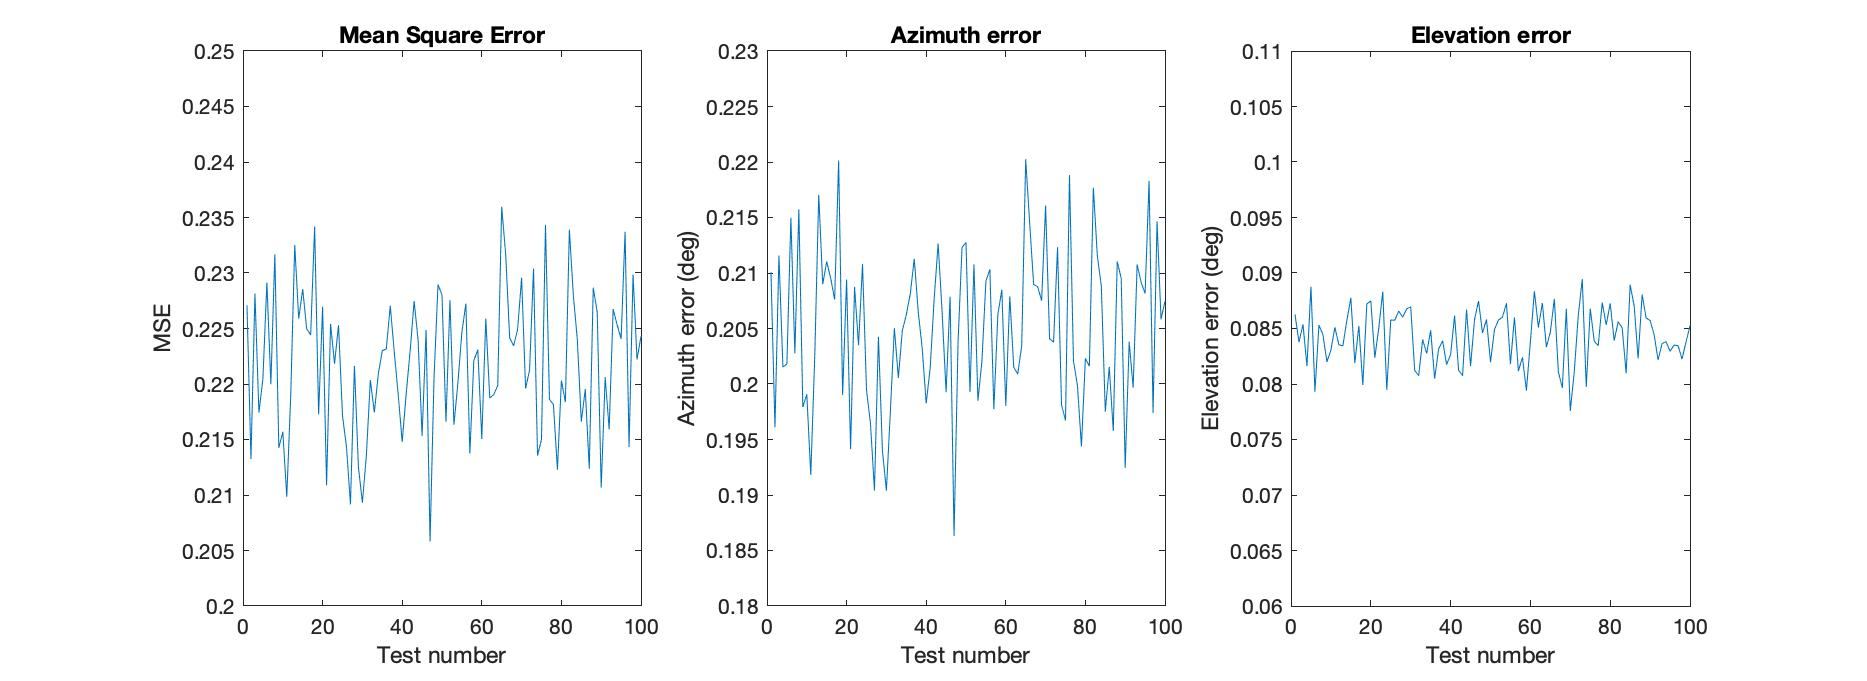
\includegraphics[width=0.9\textwidth]{figures/plot-accum0-dev0-100times}}
	\captionsetup{justification=centering,margin=2cm}
	\caption{Obtained error for a single configuration with no accumulated samples}
	\label{fig:plot-accum0}
\end{figure}

\begin{figure}[!htbp]
	\makebox[\textwidth][c]{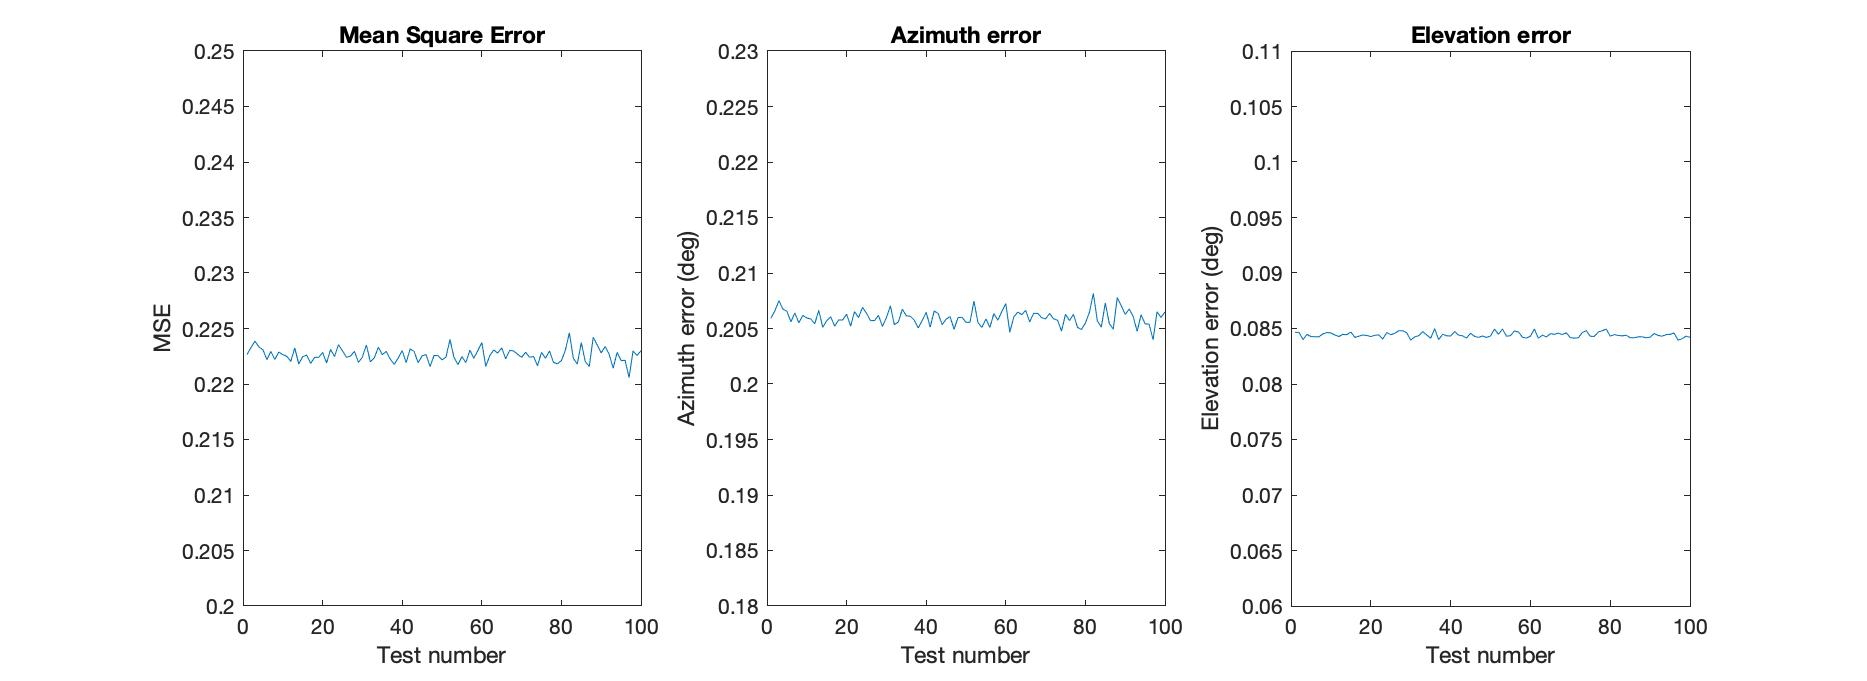
\includegraphics[width=0.9\textwidth]{figures/plot-accum100-dev0-100times}}
	\captionsetup{justification=centering,margin=2cm}
	\caption{Obtained error for a single configuration with 100 accumulated samples}
	\label{fig:plot-accum100}
\end{figure}

This approach allows to achieve more coherent results and to characterize the configurations in a more methodical manner.

\paragraph{d) Influence of increasing the configuration baseline}

Until this point, there are several mentions to the baseline of the used configuration and its numeric impact on the estimation performance. However, there are no conclusions about the optimal baseline that should be used. The goal of this test is to delineate the influence of increasing the hydrophones' baseline in the obtained error. 

In order to execute this test, configuration C is used as well as the method previously explained that reiterates each estimation a defined number of times to achieve average dispersion values. To create an increasing baseline along the tests, in each iteration the $x$ coordinate of $r_{C1}$ increases $0.01 m$ in a total of 200 times, which makes up a displacement range between 0.1 and $2 m$. Each position generates 100 accumulated samples that result in a single measurement per configuration. 

Plot \ref{fig:plot-baseline-increase-1} represents the collected errors for each of the described configurations, whose baseline is progressively increasing in a constant pace. As illustrated, the obtained errors decrease visibly in the first 100 tests, corresponding to a $r_{C1}$ position between 0.1 and $1 m$, becoming considerably constant for further distances.

\begin{figure}[!htbp]
	\makebox[\textwidth][c]{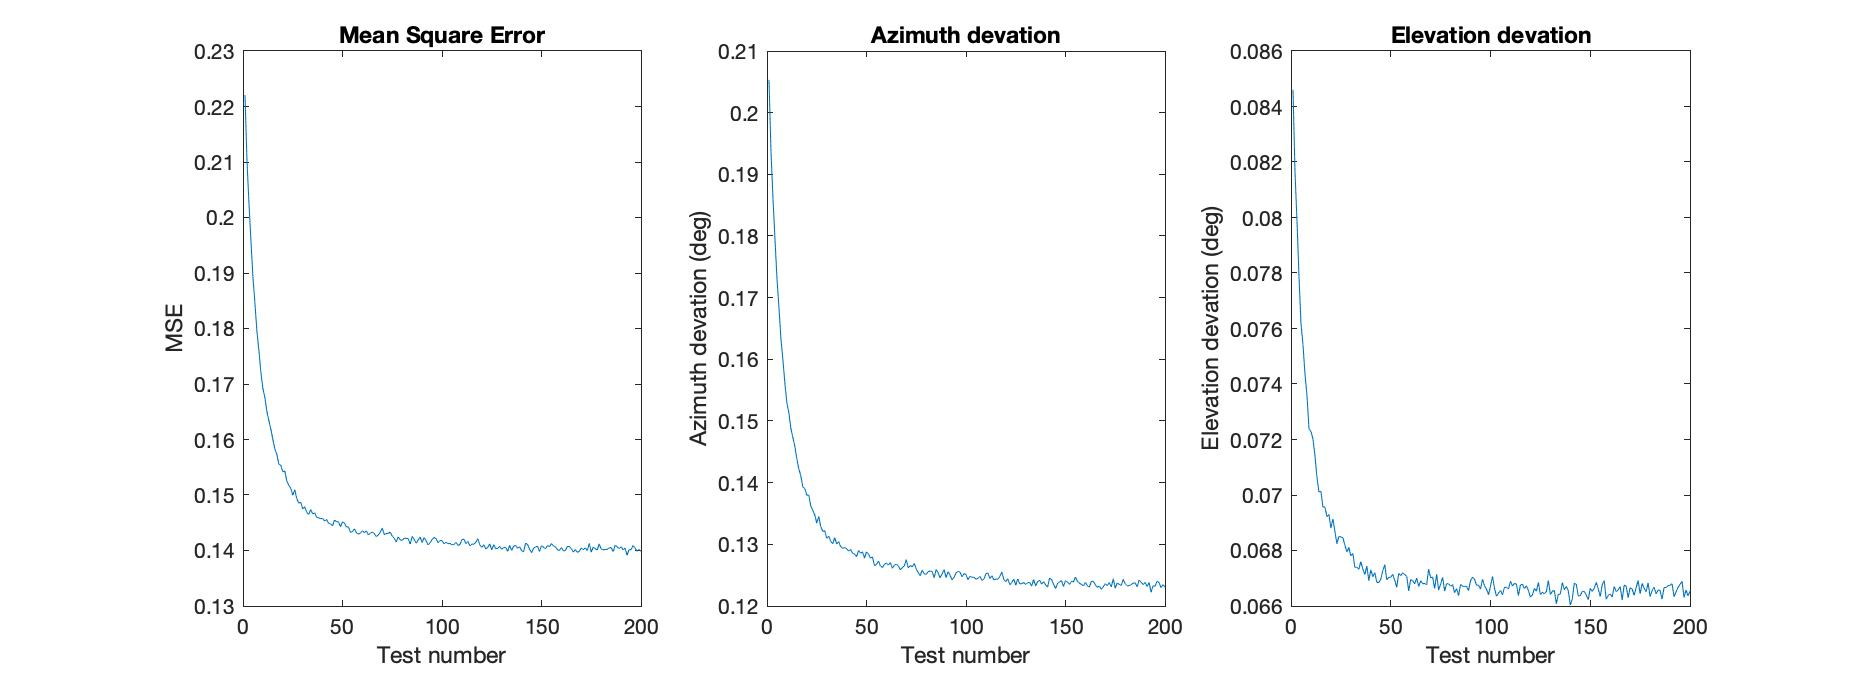
\includegraphics[width=1.1\textwidth]{figures/plot-Hbaseline-dev001-100accum-100s-1}}
	\captionsetup{justification=centering,margin=2cm}
	\caption{Error evolution with increasing baseline for $r_{C1}$}
	\label{fig:plot-baseline-increase-1}
\end{figure}

Additionally, the same experiment was done on hydrophone $r_{C2}$ of the same structure, since its position on the configuration gets a different exposure than $r_{C1}$ and a different outcome is expected. Having considered the same conditions as explained for the previous simulation, figure \ref{fig:plot-baseline-increase-2} illustrates the obtained results. It can be observed that the displacement of this specific hydrophone only causes an estimation improvement in the elevation deviation, it does not affect the estimation of the azimuth deviation and slightly increases the azimuth deviation. Therefore, an estimation improvement may not be achieved by distancing a random hydrophone, a study should be conducted for each particular configuration to determine which displacements lead to an enhancement.

\begin{figure}[!htbp]
	\makebox[\textwidth][c]{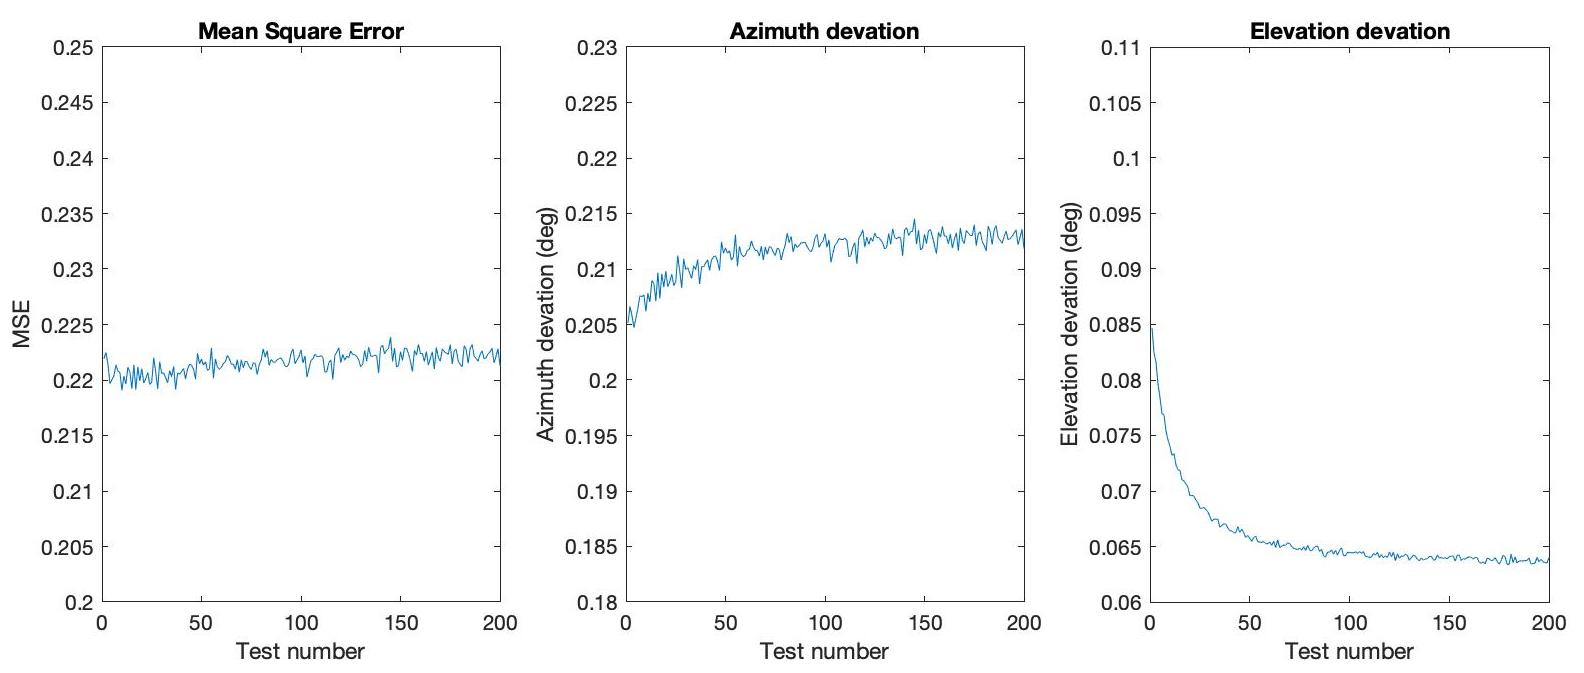
\includegraphics[width=1.1\textwidth]{figures/plot-Hbaseline-dev001-100accum-100s-2}}
	\captionsetup{justification=centering,margin=2cm}
	\caption{Error evolution with increasing baseline for $r_{C2}$}
	\label{fig:plot-baseline-increase-2}
\end{figure}

In conclusion, it is proved that increasing the baseline of a configuration in specific cases may result in a decrement of the overall estimation error. However, this only occurs for a maximum distance after which the error becomes constant. 

\paragraph{e) Conclusions on TDoA based estimator}

The present chapter focused on detailing the developed estimator, including the involved mechanisms and algorithm, a behavioral analysis and characterization based on simulated results. Therefore, by way of summary, some main conclusions can be taken:
\begin{itemize}
	\item The azimuth and elevation errors do not vary with the range of the transmitter's position, in contrast to errors in Cartesian coordinates which increase proportionally with the range;
	
	\item The ToA measurement is not essential for long range distances. So, in those cases there is no need for synchronization since a random large ToA can be used instead;
	
	\item A lower numeric precision in the calculations affects the obtained results, however since in the explored situations the errors are inherently small, the error increase does not have an impact on the system from a practical point of view;
	
	\item Increasing the baseline of a hydrophone configuration can result in a better estimation, until reaching a certain distance after which the error becomes constant. Therefore, when choosing an hydrophone layout which can be limited to the dimensions of a physical structure, it does not have to be sought the maximum baseline possible but the length that leads to the error becoming constant;
	
	\item Applying a reiteration process to create averaged errors for each configuration, creates results which are more consistent thus more capable of characterizing a specific process. Additionally, the random nature of the Monte Carlo approach is attenuated, resulting in more coherent results.
	
	\item The hydrophone configuration is a main factor on the estimation performance for any position in space. Although the characteristics that a configuration should meet to be optimal are still not clear, some aspects can be pointed out: 
	
	\begin{itemize}
		\item It is mandatory to ensure a sensor layout which covers three dimensions, so it is possible to estimate coordinates in 3D;
		\item The positions of the sensors must be linearly independent to allow the application of the least squares method;
		\item It is fundamental to have an adequate baseline which can be determined with the tool previously explained;
		\item Bearing in mind that the configuration may be employed in real scenarios, it is useful to create schematics which require achievable distances between hydrophones and respect logical shapes to install in vehicles such as AUVs.
	\end{itemize}
\end{itemize}

\subsubsection{Functional analyzes of Monte Carlo plane wavefront estimator}

In order to understand the basic behavior of the plane wavefront estimator, it was tested at first for the estimation of a single position. An injected error is considered according to the initial defined circumstances in \ref{subsec:perform-compar-meth}, which is added to the calculated ToA to each sensor. So, a series of 1000 iterations are performed to the estimation of position $s_{cart}(0,100,0)$ using configuration A and the obtained estimations are represented in \ref{fig:plot-wavefront-0,100,0-A}.

\begin{figure}[!htbp]
	\makebox[\textwidth][c]{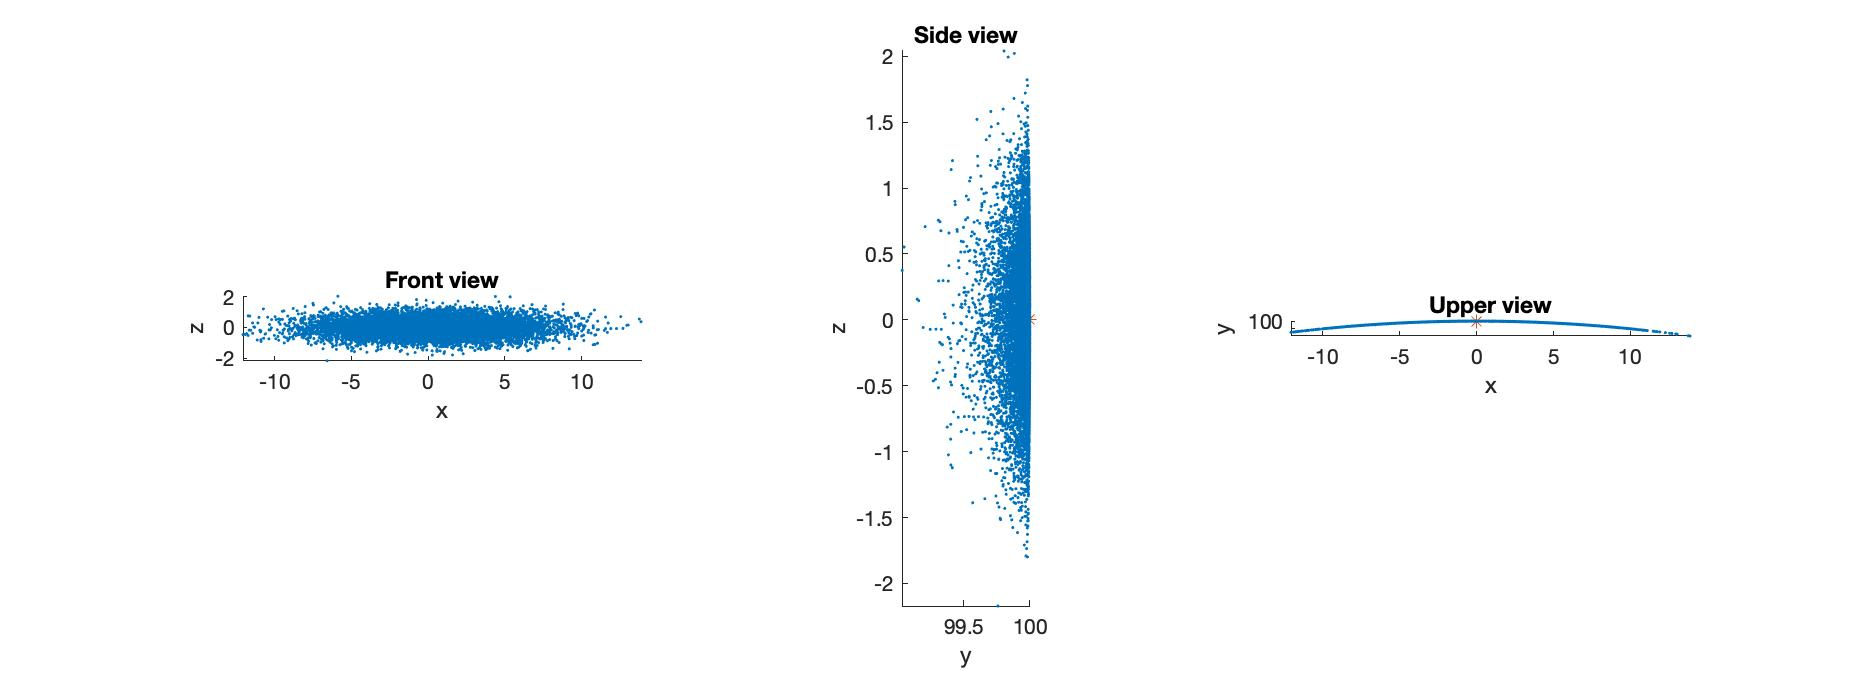
\includegraphics[width=1.1\textwidth]{figures/plot-wavefront-[0,100,0]-A}}
	\captionsetup{justification=centering,margin=2cm}
	\caption{Estimation of position $s_{cart}(0,100,0)$ using the plane wavefront estimator with configuration A}
	\label{fig:plot-wavefront-0,100,0-A}
\end{figure}

As can be observed, the upper view reveals that the estimates are placed along a sphere surface, which corresponds to the expected result since the norm is calculated as the average ToA while the direction estimation is influenced by the error that affects the TDoAs. Additionally, the front view, which represents the view from the origin to the estimated position in the y-axis, reveals a narrow estimate cloud with larger error in azimuth. However, by inspection it is possible to conclude that this relation varies according to the position that is being estimated and is not a constant proportion.

After analyzing this specific case, a second simulation intends to achieve a more comprehensive study on the performance sensor configurations. Therefore, using a specific configuration, all $s$ positions that form a sphere of defined norm were estimated a total of 1000 times, in order for the errors to be averaged, and the relevant data is retrieved, namely the standard deviation and minimum error of both azimuth and elevation estimations. The results are summarized in table \ref{tab:planewave-estimator-abc}, where configurations A, B and C are tested for norms equal to 10 and 1000 meters.

\begin{table}[!htbp] %use H to adjust
	\begin{center}
		\makebox[\textwidth]{
			\begin{tabular}{ c | c c | c c | c c}
				%\hline
				\toprule
				\multicolumn{3}{c|}{} & \multicolumn{2}{c|}{Azimuth} & \multicolumn{2}{c}{Elevation}  \\
				\midrule
				% \cline{2-9}
				\multicolumn{1}{c|}{Configuration} & Norm & MSE & Standard Dev & Minimum & Standard Dev & Minimum \\
				\midrule
				\multirow{2}{*}{A} 
				&10 	 & 0.3428 & 0.1725 & 0.2355 & 0.1713 & 0.2258 \\
				&1000 & 0.3305 & 0.1779 & 0.2334 & 0.1759 & 0.2301 \\
				\midrule	
				\multirow{2}{*}{B} 
				&10 & 0.3375 & 0.1792 & 0.2349 & 0.1739 & 0.2306 \\
				&1000 & 0.3322 & 0.1729 & 0.2336 & 0.1701 & 0.2221 \\
				\midrule			
				\multirow{2}{*}{C} 
				&10 & 0.4172 & 0.2420 & 0.3378 & 0.1797 & 0.2358 \\
				&1000 & 0.4093 & 0.2416 & 0.3218 & 0.1691 & 0.2314\\
				\bottomrule 
		\end{tabular}}
		\caption{Obtained errors for configurations A,B and C by plane wavefront estimator}
		\label{tab:planewave-estimator-abc}
	\end{center}
\end{table}

\note{table interpretation}

\subsubsection{Functional analyzes of Fisher Information Matrix}

In order to demonstrate the functionality of the described method, a first simulation was conducted in which a chosen configuration is tested for various positions $s$, returning the uncertainty sphere radius, in meters, that is obtained for each position. Similarly to what was considered before in \ref{subsec:perform-compar-meth}, for each defined norm, the elevation component covers the interval [-90$^{\circ}$ to 90$^{\circ}$] in steps of one and, for each elevation value, the azimuth component covers the interval [-180$^{\circ}$, 180$^{\circ}$] in steps of one, forming partial spheres around the reference axis' origin. The simulation was conducted using configuration C previously defined.

When estimating positions correspondent to a sphere of norm equal to $100m$, the obtained results are illustrated in figure \ref{fig:fim-100-C}, which show the uncertainty sphere radius for each of the $s$ positions, with respect to azimuth and elevation angles. The first plot represents the 3D map of each radius in relation to both angles, the second plot is a 2D view of the uncertainty with respect to the azimuth angle in degrees and the third plot is the 2D view of the uncertainty with respect to elevation angle in degrees.

\begin{figure}[!htb]
	\makebox[\textwidth][c]{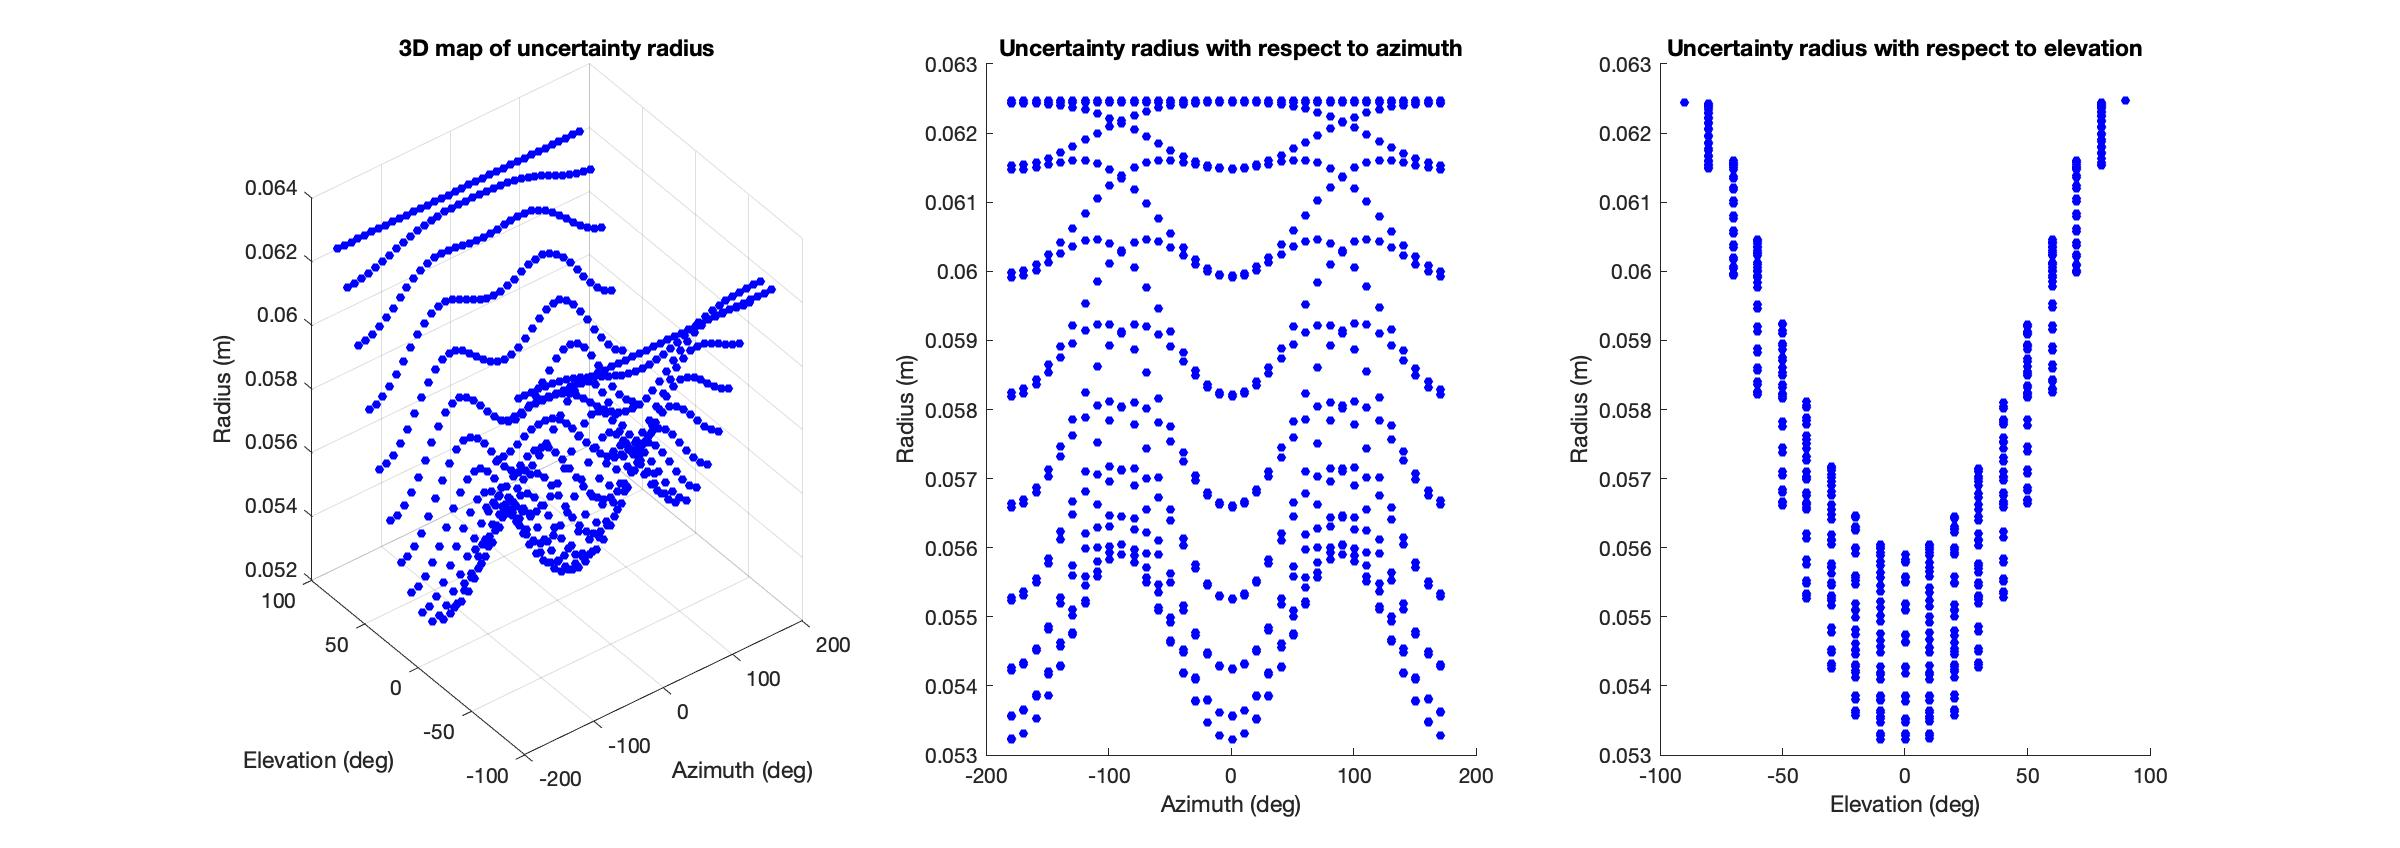
\includegraphics[width=1.2\textwidth]{figures/plot-FIM-allpos-norm100-C}}
	\captionsetup{justification=centering,margin=2cm}
	\caption{Uncertainty radius obtained by configuration C for all sphere positions}
	\label{fig:fim-100-C}
\end{figure}

In this specific case, it is noticeable that this configuration is capable of better estimations for low elevation angles and has an ascendant error for increasing elevation angles. Additionally, the uncertainty has a tendency to increase for azimuth angles around $-90^{\circ}$ and $90^{\circ}$. Overall, for a norm equal to $100 m$, the standard deviation of all estimations is $0.0029m$ and the best estimation occurred for position $s_{sph}(100,-180,3)$ in spherical coordinates, with an uncertainty radius of $0.0532m$.

This tool also makes it possible to analyze the specific uncertainty ellipsoid of a position estimate, i.e. each of the eigenvectors of the FIM, for a specific configuration. Then, resorting tho the same configuration C, it is observed that for any estimated position, the eigenvector parallel to the direction of the angle of arrival always demonstrate the smaller uncertainty. This corresponds to what is expected since the injected error affects the TDoA which has a direct influence on the angle of arrival while the ToA is estimated using absolute distances. Additionally, for any estimated position it is also observed that, if it is considered a vector connecting the origin to the transmitter position, this vector forms angles with the eigenvectors that have an approximated uniform pattern: there is always two angles which are close to $90^{\circ}$, correspondent to errors in azimuth and elevation angles, and one angle that is close to $0^{\circ}$, correspondent to the norm error. 

Figure \ref{fig:fim-eigvec-10,0,0-C} illustrates this concept for a estimation of position $s_{cart}(10,0,0)$. As indicated the first plot represents the side view, plane zx, and the third plot illustrates the view from above, plane yx, which illustrate to the norm error, the second plot represents the USBL front view, plane zy, which corresponds to the error in azimuth and elevation angle. 

\begin{figure}[!htb]
	\makebox[\textwidth][c]{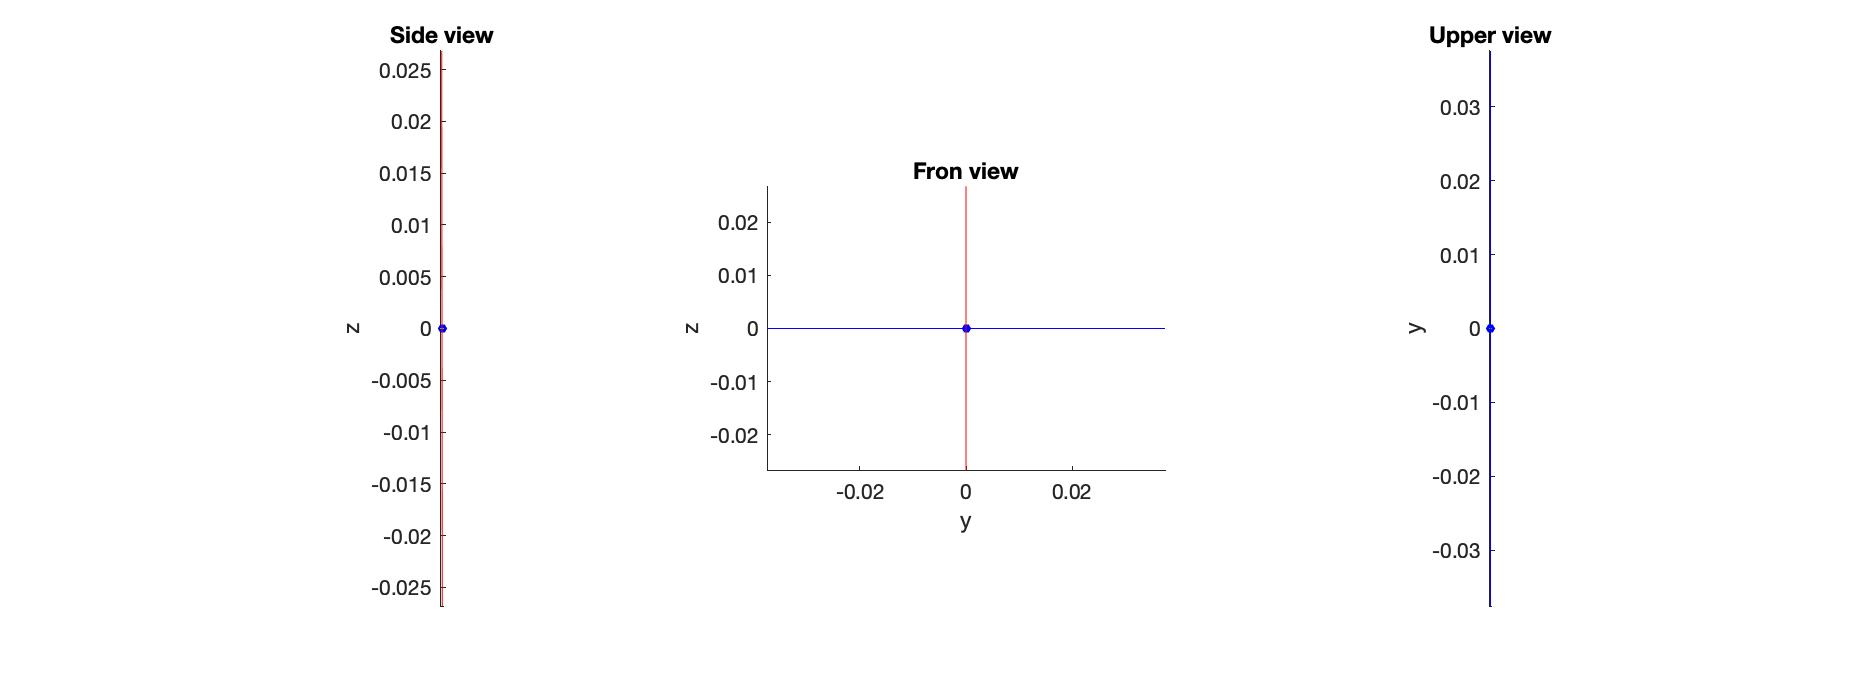
\includegraphics[width=1\textwidth]{figures//plot-fim-[10,0,0]-C}}
	\captionsetup{justification=centering,margin=2cm}
	\caption{Eigenvectors obtained for configuration C when estimation position $s_{cart}(10,0,0)$ }
	\label{fig:fim-eigvec-10,0,0-C}
\end{figure}

Finally, similarly to the previous methods a final simulation was ran on configurations A, B and C in order to evaluate their performance on the estimation of several defined positions along a sphere with norms of 10 and 1000 meters. Since the Crámer-Rao lower bound does not contemplate the azimuth and elevation errors as an optimality criteria, then other metrics are used in this case. Table  \ref{tab:fim-abc} contains the obtained data, including the criteria with the following meaning:  

\begin{itemize}
	\item \textbf{Determinant of the inverse of the FIM}: reflects the uncertainty sphere radius
	\begin{itemize}
			\item Minimum: corresponds to the smallest  uncertainty sphere radius achieved by the configuration. Represents the most accurate estimate among all estimated positions, thus an optimistic case;
			\item Maximum: corresponds to the biggest uncertainty sphere radius achieved by the configuration. Represents the estimate with lower accuracy among all estimated positions, thus a pessimistic case;
			\item Standard deviation: corresponds to the standard deviation of the obtained determinants of the inverse of the FIM for all estimated positions. Reflects the variance of the estimates.
	\end{itemize}
	\item \textbf{ Maximum Eigenvalue of the inverse of the FIM}: considering the uncertainty ellipsoid, which presents three uncertainty axis with distinct magnitudes, this parameter reflects the maximum uncertainty that is achieved for each position
	\begin{itemize}
			\item Minimum: considering that each configuration obtains a maximum eigenvalue for each estimated position, this parameters corresponds to the position whose largest uncertainty is minimized.
	\end{itemize}
	\item \textbf{Trace of the inverse of the FIM}: reflects the sum of the magnitudes of the uncertainty axis for each estimated position
	\begin{itemize}
			\item Minimum: corresponds to the minimum of the uncertainty average variance, thus the positions that reveals a the lowest summed uncertainty magnitudes
	\end{itemize}
\end{itemize}


\begin{table}[!htbp] %use H to adjust
	\begin{center}
		\makebox[\textwidth]{
			\begin{tabular}{ c | c | c c c | c | c }
				%\hline
				\toprule
				\multicolumn{2}{c|}{} & \multicolumn{3}{c|}{Determinant} & \multicolumn{1}{c|}{Max Eigenvalue} & \multicolumn{1}{c}{Trace}  \\
				
				\midrule
				\multicolumn{1}{c|}{Configuration} & Norm & Min & Max & Std & Min & Min\\
				
				\midrule
				\multirow{2}{*}{A} 
				& 10 	 & 0.010 & 0.0200 & 0.003 & 0.053 & 5.6$\times10^{-3}$  \\
				& 1000 & 0.220 & 0.421 & 0.067 & 5.310 & 56.325 \\
				
				\midrule	
				\multirow{2}{*}{B} 
				& 10 	 & 0.010 & 0.011 & 3.8$\times10^{-4}$ & 0.0530 & 5.6$\times10^{-3}$ \\
				& 1000 & 0.2193 & 0.2462 & 0.008 & 5.306 & 56.283 \\
				
				\midrule			
				\multirow{2}{*}{C} 
				& 10 	 & 0.012  & 0.014 & 6.3$\times10^{-4}$ & 0.075 & 8.5$\times10^{-3}$  \\
				& 1000 & 0.247 & 0.290 & 0.014 & 7.410 & 84.882 \\
				\bottomrule 
		\end{tabular}}
		\caption{Obtained errors for configurations A,B and C by Crámer-Rao lower bound}
		\label{tab:fim-abc}
	\end{center}
\end{table}


\subsection{Final remarks}

This section was dedicated to the implemented hardware design for FPGA technology and a comprehensive study on evaluation tools for the performance of sensor configurations. From this, we may draw some conclusions.

\note{compare tables 4.3, 4.4, 4.5\\draw conclusions}

The plane wavefront estimator demonstrates better performance for long range estimation, since the considered approximation is only valid for large distances. 

For short range, the TDoA estimator demonstrates better performance than the latter, since the TDoA values, which are very precise, are more relevant for the calculation.

Overall, the Crámer-Rao lower bound is a method widely used for performance evaluation. The Fisher Information Matrix reflects the quantity of information that a configuration is capable of acquiring in relation to a specific position, which is directly associated with the accuracy of the estimation.  Therefore, it is considered the most reliable mechanism for this study. 
